%Chapter "Introduction"
%
\chapter{Introducción a los Elementos Finitos}
\graphicspath{{img/FEM/}}

\section{Presentación}

Como se mencionó anteriormente, en la práctica se requiere de métodos numéricos
para resolver las ecuaciones resultantes de un problema de interés. Por ejemplo,
la figura \ref{fig:chirajara} presenta el primer modo de pandeo para un pilón 
del puente Chirajara que se obtuvo usando el método de elementos finitos, 
realizado por estudiantes de la materia en 2018 \cite{pandeo_chirajara}. Basados
en este análisis los autores obtuvieron que la carga  crítica para el pilón
es alrededor de 2.24 veces su peso, mientras que para una columna de sección 
cuadrada y relación de aspecto de 10 la carga es alrededor de 370 veces su peso.
\begin{figure}[h]
    \centering
    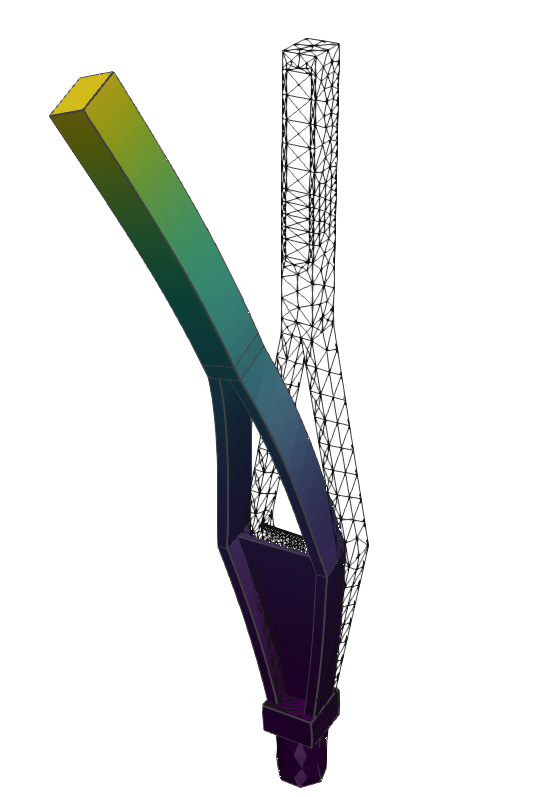
\includegraphics[width=6 cm]{pandeo_chirajara.png}
    \caption{Primer modo de pandeo para un pilón del puente Chirajara. Se 
    presenta la configuración deformada y la configuración original como 
    referencia. La carga crítica para este pilón es alrededor de 2.24 veces
    el peso de la estructura.}
    \label{fig:chirajara}
\end{figure}

\subsection{Introducción}

El método de los elementos finitos es una técnica numérica para la solución de 
problemas de valores en la frontera propuesta inicialmente a finales de los 50 
y principios de los 60  \cite{clough65, turner56}. Desde entonces, ha 
experimentado un fuerte desarrollo tecnológico y académico, plasmado en una 
gran cantidad de paquetes comerciales y de aplicaciones en diferentes áreas de 
ciencia e ingeniería. Paralelamente, se han escrito una gran cantidad de textos 
cubriendo aspectos teóricos relativos a la formulación y a la implementación 
del método \cite{book:bathe, book:hughes,  book:reddy, book:zienkiewicz}. En la 
actualidad el método de los elementos finitos puede considerarse como la 
herramienta de simulación numérica más poderosa y versátil para el estudio de 
problemas de ingeniería. 

Desde el punto de vista teórico el método se basa en la solución de la forma 
débil del problema de valores en la frontera sobre una discretización del 
dominio en elementos finitos en cada uno de los cuales se expresa la solución 
usando interpolación a partir de valores determinados para unos cuantos puntos 
o nodos. La contribución de cada elemento finito del dominio es posteriormente 
sumada usando leyes gobernantes entre las diferentes variables del problema. En 
el caso mecánico la forma débil del problema de valores en la frontera 
corresponde al principio de los desplazamientos virtuales y el ensamblaje o 
consideración de todos los elementos se construye a partir de condiciones de 
equilibrio y compatibilidad de desplazamientos. 

En ingeniería civil el método de elementos finitos es aplicable en la 
simulación de problemas relativos a áreas como mecánica de fluidos, análisis 
dinámico de estructuras, mecánica de suelos, análisis de presas, o estructuras 
de contención. Algunos programas comerciales, específicamente desarrollados 
para uso en ingeniería civil son:  
Plaxis\footnote{\url{http://www.plaxis.nl/plaxis2d/}}, 
SAP2000\footnote{\url{https://www.csiamerica.com/products/sap2000}}, 
OpenSees\footnote{\url{http://opensees.berkeley.edu/wiki/index.php/Main_Page}}.

A pesar del gran desarrollo del método y de su amplio uso en oficinas de 
ingeniería, especialmente en países desarrollados, este no es impartido en los 
currículos de ingeniería civil en la mayoría de universidades colombianas. En 
este capítulo se hace uso de un programa por elementos finitos desarrollado en 
Python y dirigido al análisis de sólidos elásticos en condiciones de tensión 
plana y deformación plana. El programa ha sido desarrollado principalmente con 
fines educativos en los cursos IC0285 Modelación Computacional y IC0602 
Introducción al Método de los Elementos Finitos de la Universidad EAFIT. El 
software es libre y de código abierto\footnote{La licencia es 
\href{https://opensource.org/licenses/MIT}{MIT} y puede descargarse del 
siguiente enlace: \url{https://github.com/AppliedMechanics-EAFIT/SolidsPy}.}. 
Paquetes similares, desarrollados en Python y dirigidos a uso educativo pueden 
identificarse en las herramientas SfePy \cite{sfepy}, PyFEM \cite{pyfem} and 
FEniCS \cite{fenics}.

\subsection{Aplicaciones de los elementos finitos}

El rango de aplicaciones de los elementos finitos es muy diverso, para brindar una idea de su versatilidad se presenta la siguiente lista \cite{book:first_fem}:
\begin{itemize}
	\item análisis térmico y de esfuerzos en partes industriales como circuitos integrado, dispositivos electrónicos, válvulas, tuberías, tanques, motores de autos y aviones;
	\item análisis sísmico de presas, plantas eléctricas, ciudades y edificios altos;
	\item análisis de choques de carros, trenes y aviones;
	\item análisis del flujo de contaminantes y sistemas de ventilación;
	\item análisis electromagnético de antes, transistores y aviones;
	\item análisis de procedimientos quirúrgicos como cirugías plásticas, reconstrucción de quijadas, corrección de escoliosis y muchas otras.
\end{itemize}

El uso de análisis por elementos finitos de estructuras ha reducido los ciclos de diseño considerablemente y mejorado la calidad de los productos en general. 


\section{Concepto intuitivo de rigidez}
Uno de los aspectos fundamentales para el estudio del método de elementos
finitos en problemas de mecánica es el de rigidez. A continuación se presenta
de manera intuitiva este concepto.

Considere los 2 modelos mostrados en la siguiente figura. El primero 
corresponde a un resorte de constante $k$ el cual tras ser sometido a la acción 
de una fuerza externa $F$ experimenta un cambio en su longitud igual a 
$\delta$. El mismo problema se ilustra en el modelo abstracto de un sólido 
representado por la `papa' y en el cual la línea continua describe la forma de 
la `papa' antes de aplicar la fuerza externa $F$, mientras que la línea 
punteada describe la forma de la `papa' tras aplicar la fuerza. Los apoyos 
esquemáticos (de triángulo y rodillo) que se muestran en la figura 
\ref{fig:rigidez} indican que la `papa' no se podrá desplazar como un cuerpo 
rígido.

\begin{figure}[H]
\centering
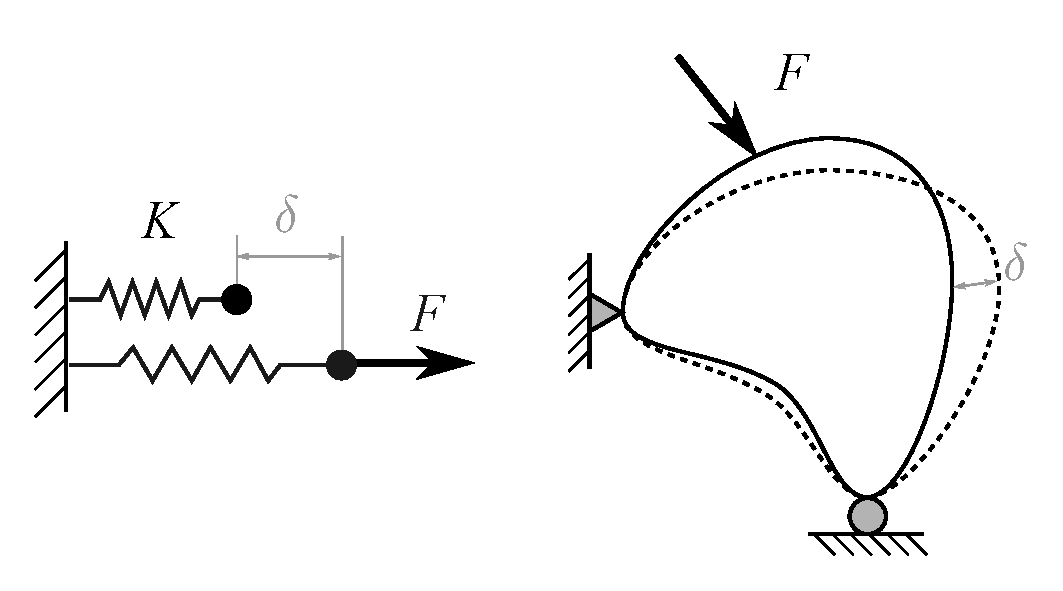
\includegraphics[width=12cm]{rigidez.pdf}
\caption{Esquema del concepto de rigidez, se hace una analogía entre la 
deformación de un resorte de constante $k$ , y la deformación que sufre un 
cuerpo ante cierta carga.}
\label{fig:rigidez}
\end{figure}

En el resorte se satisface la relación:
\begin{equation*}
F = k \delta
\end{equation*}
y en la cual el coeficiente de rigidez $k$ representa la fuerza necesaria para 
producir un desplazamiento unitario $\delta = 1.0$.

En el caso de la `papa', el problema es más complejo ya que existen muchas 
direcciones posibles y puntos en los cuales aplicar las fuerzas y en los cuales 
medir los desplazamientos. ¿Cómo podemos cuantificar la rigidez para este caso?

Sea $\delta _i$ el desplazamiento en un punto cualquiera medido en una 
dirección $i$ y sea $F_j$ la fuerza aplicada en la dirección $j$ también en un 
punto arbitrario de la `papa'. En este caso siguiendo la idea del resorte es 
posible escribir:

\begin{equation*}
F_j = k \delta_i\, .
\end{equation*}

Comparando esta relación con la correspondiente al problema del resorte se 
puede concluir que el coeficiente $k$ representa la fuerza necesaria a lo largo 
de la dirección $j$ para producir un desplazamiento unitario en la dirección 
$i.$


Nótese que si se cambia la dirección en la que se aplica la fuerza y la 
dirección en la que se mide el desplazamiento es esperable que el coeficiente 
de rigidez también cambie. Por lo tanto un modelo mas general sería:

\begin{equation}
F_j = k_{ji} \delta_i\, .
\end{equation}

y en el cual los subíndices $ij$ dan cuenta de que el coeficiente de rigidez 
$k_{ij}$ representa la fuerza necesaria a lo largo de la dirección $j$ para 
producir un desplazamiento unitario en la dirección $i.$

\subsection{¿Cómo describir el sólido?}

El modelo propuesto para el caso del sólido es físicamente correcto pero 
operativamente existen infinitas direcciones posibles $i$ y $j$ y surge 
entonces la pregunta: \textbf{¿cómo cuantificar la rigidez para el caso de la 
`papa'?}

Consideremos algunas posibles soluciones:
\begin{enumerate}
    \item Solución discreta: Aproximar el sólido mediante un sistema finito de 
    partículas conectadas por resortes.
    \item Solución del continuo: Estudiar el comportamiento de un elemento 
    diferencial generando un sistema de ecuaciones diferenciales (en las 
    variables $u_i$, $\epsilon_{ij}$ y $\sigma_{ij}$).
    \item Solución numérica: Combinar \textbf{1} y \textbf{2} para hacer una 
    aproximación discreta del continuo (métodos por elementos finitos). La 
    comparación entre las soluciones \textbf{1} y \textbf{2} se describe en la 
    siguiente tabla:
\end{enumerate}
%
\begin{table}[H]
\begin{tabular}{p{6cm}p{6cm}}
\hline
\textbf{Planteamiento del continuo} & 
\textbf{Planteamiento discreto}\\
\hline
Número infinito de elementos diferenciales por resortes.
& Número finito de partículas conectadas por resortes.\\
Desplazamientos, deformaciones y tensiones.
& Desplazamientos y fuerzas.\\
\hline
\end{tabular}
\end{table}


\subsection{Elementos finitos (aproximando el continuo)}
La figura muestra nuevamente el problema esquemático de la `papa'. Esta ha sido 
dividida en un número \textbf{finito} de triángulos conectados en las esquinas. 
Cada triángulo esta definido por 3 puntos correspondientes a sus vértices. 
Denominemos un triangulo típico como $\Omega_e$. Asuma que cada vértice del 
triángulo típico $\Omega_e$ se comporta como una partícula y que esta puede 
experimentar desplazamientos (y fuerzas) en la dirección horizontal y vertical. 
Asuma además que para el triángulo típico las 3 partículas que lo definen están 
conectadas por resortes.
\begin{figure}[H]
\centering
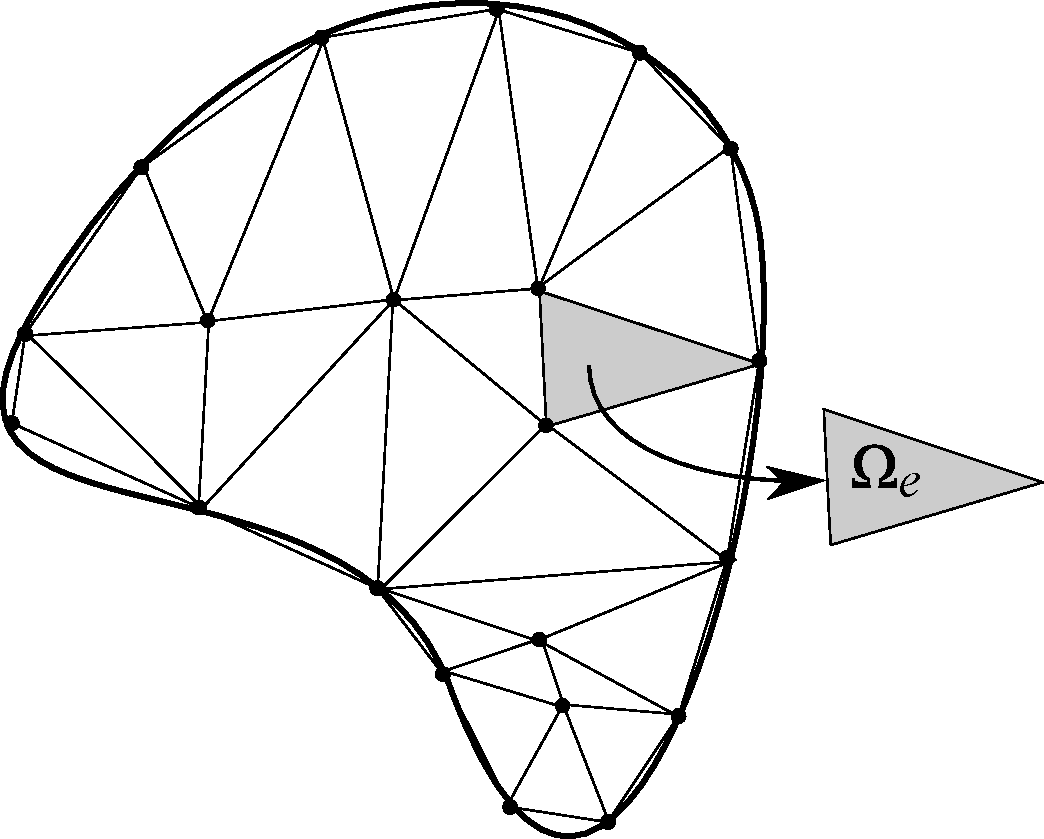
\includegraphics[width=8cm]{dominio_discreto.pdf}
\caption{Esquema de la discretización del dominio arbitrario en un conjunto 
finito de elementos triangulares.}
\label{fig:meshed}
\end{figure}

\section{Relación fuerza-desplazamiento para todo el sistema}
Se tiene entonces que para un triangulo típico $\Omega_e$ es posible relacionar 
las 6 fuerzas con los 6 desplazamientos mediante una ecuación general como:
\begin{equation}
F_j = k_ {ji} \delta_i
\end{equation}

y en la cual el término $k_{ji}$ representa 36 coeficientes de rigidez. Si se 
considera que el índice $j$ puede tomar 6 valores correspondientes a 6 fuerzas 
y que el índice $i$ puede tomar 6 valores correspondientes a 6 desplazamientos 
entonces se puede reconocer que se tiene un sistema de 6 ecuaciones el cual 
podemos escribir matricialmente como:
\begin{equation}
\{ F \}=[ K ] \{ u \}\, .
\end{equation}

De manera similar, es posible anticipar que es posible escribir una relación 
que considere todos los puntos del dominio. Por ejemplo, si se tienen $N$ 
puntos en total habrán $2N$ fuerzas y $2N$ desplazamientos. Escribamos la 
relación entre fuerzas y desplazamientos para todo el sólido (representado por 
$N$ puntos) como:

\begin{equation}
F_j^G = k_ {ji}^G \delta_i\, .
\end{equation}

En esta relación hemos usado el superíndice $G$ para enfatizar que las fuerzas, 
desplazamientos y coeficientes de rigidez corresponden a todo el sólido y no a 
un elemento típico. En forma matricial se tiene:

\begin{equation}
\{ F^G \} = [ K^G ] \{ U^G \}\, .
\end{equation}

El superínidce $G$ también indica que las ecuaciones son válidas para todo el 
sistema global representado por todos los triángulos en los que ha sido 
dividido el sólido.

De acuerdo con la discusión anterior, tanto el equilibrio de un triángulo 
típico $\Omega_e$ como el de un resorte pueden formularse mediante una relación 
fuerza-desplazamiento de la forma:

\begin{equation}
\{ F \} = [ K ] \{ u \}\, .
\end{equation}

En el caso del resorte es sencillo determinar la matriz de rigidez $[K]$.

En el caso del sólido el problema es un poco más elaborado y por el momento nos 
conformaremos con suponer que esta matriz se encuentra disponible. En cualquier 
caso, sea que se trata de un sistema de partículas conectadas por resortes, o 
un sólido representado por triángulos, el problema se resuelve ensamblando la 
matriz de rigidez global $[K^G]$ y resolviendo el sistema de ecuaciones:

\begin{equation}
\{ F^G \} = [ K^G ] \{ U^G \}\, .
\end{equation}

A continuación se discute con más detalle el problema usando un sistema de 
partículas unidas por resortes y se implementa su solución en el computador.

\subsection{Sistema partícula-resorte}
El siguiente ejemplo permite entender desde un punto de vista físico el proceso 
de solución del problema de varias partículas interactuando a través de un 
sistema de resortes como el que se muestra en la figura 
\ref{fig:sistema_resortes}.
\begin{figure}[H]
\centering
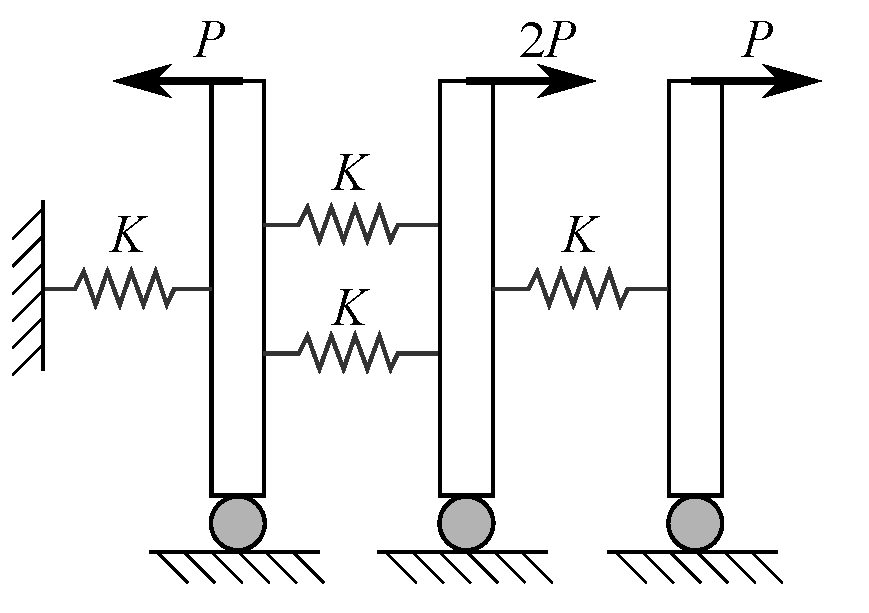
\includegraphics[width=10cm]{sistema_resortes.pdf}
\caption{Sistema de masas y resortes acoplados.}
\label{fig:sistema_resortes}
\end{figure}

El sistema de varias partículas se encuentra conectado por resortes con 
coeficiente de rigidez $k$. El sistema se encuentra sometido a diferentes 
fuerzas externas (representadas en múltiplos de $P$). Por efectos de 
visualización las partículas se representan como carritos rectangulares.

Se requiere:

\begin{enumerate}

\item
Plantear las ecuaciones de equilibrio para una partícula típica mostrada en 
la figura \ref{fig:dcl_masa}. Asuma que la partícula esta conectada a un 
resorte $i$ por la izquierda y a un resorte $i+1$ por la derecha de manera que 
el diagrama de cuerpo libre para la partícula es como el que se muestra en la 
figura \ref{fig:dcl_masa}.

\begin{figure}[H]
\centering
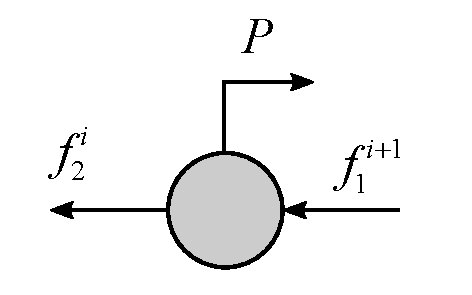
\includegraphics[width=6cm]{dcl_masa.pdf}
\caption{Diagrama de cuerpo libre para una partícula típica.}
\label{fig:dcl_masa}
\end{figure}

\item
Plantear las relaciones fuerza-desplazamiento para el resorte típico 
mostrado en la figura \ref{fig:elemento_resorte}. En esta los subíndices 1 y 2 
hacen referencia a las fuerzas y desplazamientos de los puntos 1 y 2 que 
definen el resorte.
\begin{figure}[H]
\centering
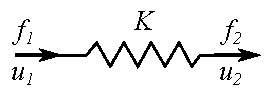
\includegraphics[width=6cm]{elemento_resorte.pdf}
\caption{Diagrama de las relaciones fuerza-desplazamiento en un resorte 
típico.}
\label{fig:elemento_resorte}
\end{figure}

\item
Enumerar las partículas y resortes del sistema. (Asumir el empotramiento 
como una partícula).

\item
Escribir las ecuaciones de equilibrio para cada una de las 4 partículas.

\item
Usando las relaciones fuerza-desplazamiento de los diferentes resortes 
re-escribir las ecuaciones del numeral \textbf{4}.

\end{enumerate}

\section{Algoritmo de solución}

En la solución del problema anterior se usaron planteamientos mecánicos para 
formular las ecuaciones de equilibrio del sistema de partículas. Consideremos 
ahora su solución de una manera sistemática de tal forma que el problema se 
pueda codificar en un programa general de análisis estructural.

\subsection{Equilibrio de los resortes}

Considere el siguiente sistema de 3 partículas, las cuales están conectadas por 
resortes $i$ e $i+1$ con coeficientes de rigidez $K^i$ y $K^{i+1}$. De manera 
similar, las partículas tienen asignados los nombres $j-1$, $j$ y $j+1$ y sus 
respectivos desplazamientos se denotan por $u_{j-1}$, $u_{j}$ y $u_{j+1}$.
\begin{figure}[H]
\centering
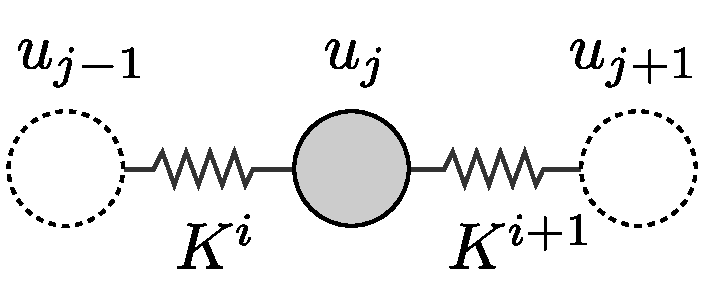
\includegraphics[width=10cm]{ibc.pdf}
\caption{Esquema de sistema de 3 partículas conectadas por resortes.}
\label{fig:ibc}
\end{figure}


Escribamos las ecuaciones de equilibrio para los resortes $i$ e $i+1$ en 
términos de los desplazamientos $u_{j - 1}$, $u_j$ y $u_{j + 1}$ como:
$$\begin{Bmatrix} f_1^i\\ f_2^i \end{Bmatrix}
= \begin{bmatrix}
k_{11}^i & k_{12}^i\\
k_{21}^i & k_{22}^i
\end{bmatrix}
\begin{Bmatrix} u_{j - 1}\\ u_j \end{Bmatrix}\, ,$$
y
$$\begin{Bmatrix} f_1^{i + 1}\\ f_2^{i + 1}\end{Bmatrix}
= \begin{bmatrix}
k_{11}^{i + 1} & k_{12}^{i + 1}\\
k_{21}^{i + 1} & k_{22}^{i + 1} \end{bmatrix}
\begin{Bmatrix} u_j\\ u_{j + 1} \end{Bmatrix}\, .$$

Note que hemos usado notación fila-columna en los índices para los coeficientes 
de rigidez para simplificar su implementación en el computador.


\subsection{Equilibrio de una partícula}
Asumiendo que la partícula $j$ se encuentra sometida a una carga externa $P$, 
se tiene, de su diagrama de cuerpo libre, que:
$$
k_{21}^i u_{j - 1} + (k_{22}^i + k_{11}^{i + 1}) u_j + k_{12}^{i + 1} u_{j + 1} 
= P_j.
$$

Procediendo de manera similar para las partículas ${j-1}$ y ${j+1}$ y 
considerando la contribución de los resortes $K^i$ y $K^{i+1}$ obtenemos el 
siguiente bloque del sistema completo de ecuaciones:
$$\begin{bmatrix}
k_{11}^i &k_{12}^i &0\\
k_{21}^i &k_{22}^i + k_{11}^{i + 1} &k_{12}^{i + 1}\\
0 &k_{21}^{i + 1} &k_{22}^{i + 1}
\end{bmatrix}\, . $$

Al considerar el sistema completo de partículas y resortes se obtiene un 
sistema de ecuaciones lineales de la forma general:
$$
[K_G] \{U_G\}  = \{F_G\}\, .
$$

En este sistema cada ecuación representa el equilibrio de una partícula.

\subsection{Ensamblaje}
La construcción de las matrices globales que describen el equilibrio de cada 
masa (o partícula) en el sistema puede programarse en el computador mediante un 
algoritmo que considere el aporte (en términos de fuerzas) de cada elemento (o 
resorte).

A este proceso se le denomina como \textbf{Ensamblaje} de las ecuaciones 
globales. La operación de ensamblaje puede realizarse después de identificar la 
conexión entre los (desplazamientos o) grados de libertad globales y los 
(desplazamientos o) grados de libertad locales mediante una matriz que almacena 
en cada fila los identificadores de los grados de libertad globales asociados a 
cada elemento.

Por ejemplo, en el sistema de 3-partículas los resortes $i$ y $i+1$ tienen como 
desplazamientos de sus extremos los denotados como $u_{j-1}$ y $u_j$ y $u_j$ y 
$u_{j+1}$. Dichos índices contienen toda la información necesaria para realizar 
el ensamblaje. La matriz que almacena los índices globales para todos los 
elementos en el modelo es la matriz \textit{DME} dada por:

$$ DME = \begin{bmatrix}
j - 1 &j\\
j &j + 1\\
\end{bmatrix}\, .$$

Nótese que en esta matriz los datos de la primera fila mostrada son $j - 1$ y 
$j$, los cuales corresponden a los identificadores de los grados de libertad 
asociados con el resorte $i$. De la misma manera los datos de la segunda fila 
mostrada son $j$ y $j+1$ los cuales corresponden a los identificadores de los 
grados de libertad asociados con el resorte $i+1$.

Una vez se tiene disponible la matriz \emph{DME}, el proceso de ensamblaje se 
realiza como se describe a continuación:
\begin{align*}
&K_{j - 1,j - 1} \leftarrow K_{j - 1,j - 1} + k_{11}^i\\
&K_{j - 1,j} \leftarrow K_{j - 1,j} + k_{12}^i\\
&K_{j,j - 1} \leftarrow K_{j,j - 1} + k_{21}^i\\
&K_{j,j} \leftarrow K_{j,j} + k_{22}^i
\end{align*}
y
\begin{align*}
&K_{j,j} \leftarrow K_{j,j} + k_{11}^{i + 1}\\
&K_{j,j + 1} \leftarrow K_{j,j + 1} + k_{12}^{i + 1}\\
&K_{j + 1,j} \leftarrow K_{j + 1,j} + k_{21}^{i + 1}\\
&K_{j + 1,j + 1} \leftarrow K_{j + 1,j + 1} + k_{22}^{i + 1}
\end{align*}


Note la conexión entre los índices locales, correspondientes a $1$ y $2$, y las 
posiciones en la matriz global, correspondientes a $j-1$, $j$ y $j+1$.


\subsection{Ejemplo de ensamblaje}
A continuación se muestra el paso a paso del ensamble de la matriz global de 
rigidez para el sistema mostrado a continuación:
\begin{figure}[H]
    \centering
    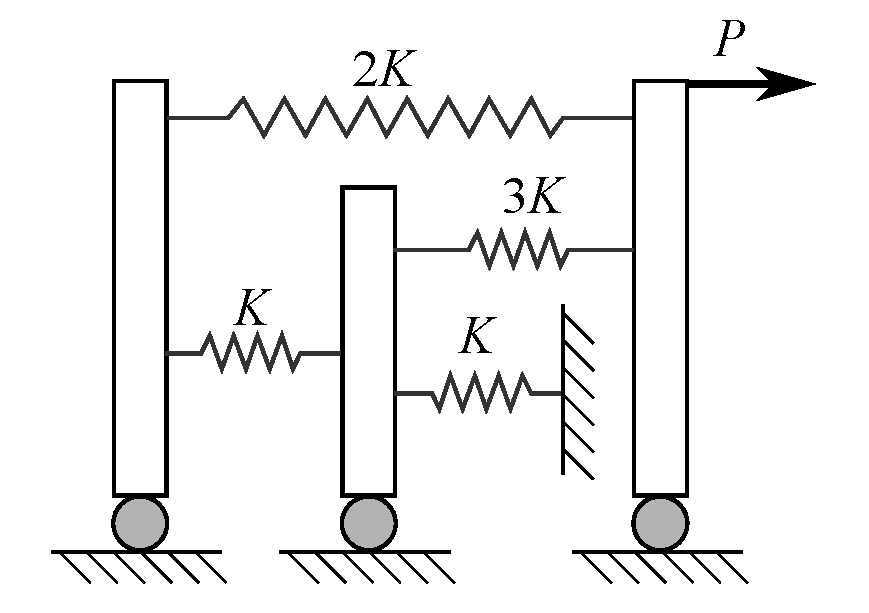
\includegraphics[width=8cm]{sistema_resortes2.pdf}
\end{figure}

El primer paso a llevar a cabo es etiquetar los nodos (masas), y los elementos 
(resortes) existentes en el sistema. Dichas etiquetas se muestran en la figura 
a continuación:
\begin{figure}[H]
    \centering
    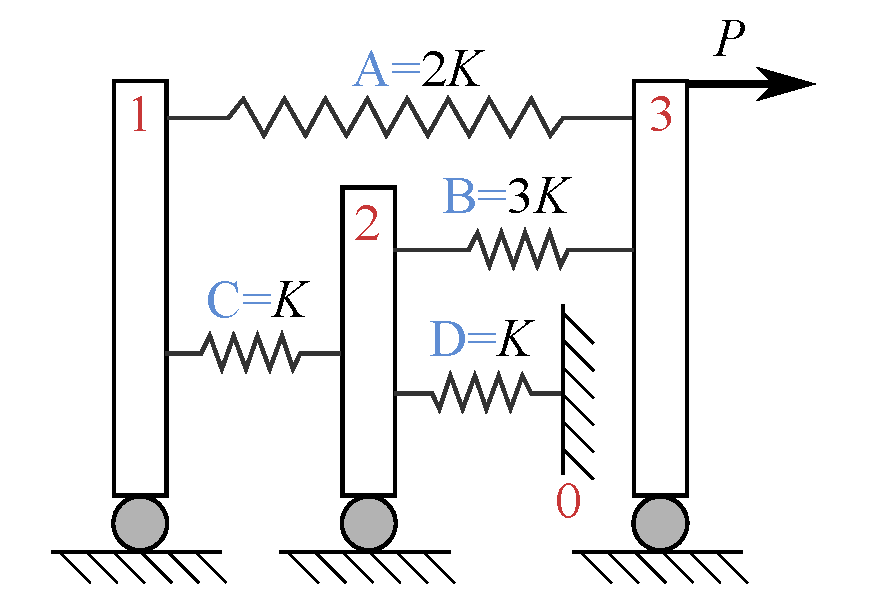
\includegraphics[width=8cm]{sistema_resortes2_etiquetas.pdf}
\end{figure}
donde los nodos se muestran en rojo, y se enumeran de 0 a 3, mientras que los 
elementos se marcan en azul oscuro, con letras desde la A hasta la D. Note que 
el empotramiento también se cuenta como nodo.

El siguiente paso es extraer, a partir del sistema, las matrices IBC (en su 
primera y segunda versión), y la matriz IELCON.

Recordemos que la matriz IBC tiene tantas filas como nodos tiene el sistema (en 
este caso tiene 4 nodos), y tantas columnas como grados de libertad tiene cada 
nodo (en este caso cada nodo tiene 1 grado de libertad ya que solo se puede 
mover horizontalmente). Y en cada posición de la matriz se pone -1 si el grado 
de libertad de dicho nodo se encuentra restringido, y 0 en caso contrario. Con 
todo lo anterior, la matriz IBC (al menos en su primera versión) es:
$$IBC = 
\begin{bmatrix}
-1 \\ 
0 \\
0 \\
0
\end{bmatrix}\, ,
$$
esto quiere decir que el nodo 0 (fila 0 de la matriz) está empotrado, 
mientras que los otros nodos están libres, tal como se muestra en la figura.

La segunda versión de la matriz IBC consiste en enumerar los grados de libertad 
que estén libres, es decir, aquellos con cero:
$$IBC = 
\begin{bmatrix}
-1 \\
0 \\
1 \\
2
\end{bmatrix}
$$

Note que, de esta forma, cada grado de libertad queda asociado a un número 
particular. Dicha segunda versión de la matriz IBC corresponde a la salida IBC 
de la función \textit{eqcounter} de los Notebooks previamente mencionados.

Por otra parte, armemos la matriz IELCON a partir del sistema en cuestión. En 
este caso, la matriz tiene tantas filas como elementos tiene el sistema (en 
este caso 4 elementos), y tiene tantas columnas como nodos asociados tenga cada 
elemento. En el caso de los resortes a trabajar, se tienen 2 nodos asociados 
(uno en cada punta).

Con lo anterior, la matriz IELCON es la siguiente:
$$IELCON = 
\begin{bmatrix}
1 & 3 \\
2 & 3 \\
1 & 2 \\
2 & 0 
\end{bmatrix}
$$

Note que la primera fila corresponde al elemento A, que conecta a los nodos 1 y 
3, mientras que la segunda corresponde al elemento B, que une los nodos 2 y 3, 
y así sucesivamente.

A partir de las matrices IBC e IELCON, se construye la matriz DME. Para 
entender esto, primero reconozcamos que cada nodo tiene un número asociado y 
registrado en la matriz IBC. Entonces, para generar la matriz DME basta con 
tomar la matriz IELCON e intercambiar los números de los nodos en esta, por los 
números asociados a estos de acuerdo con la matriz IBC. 

Es decir, en la matriz IELCON vamos a cambiar 0 por -1, 1 por 0, 2 por 1 y 3 
por 2, así:
$$DME = 
\begin{bmatrix}
0 & 2 \\
1 & 2 \\
0 & 1 \\
1 & -1 
\end{bmatrix}
$$

Note que esta matriz es la salida DME\_mat de la función \textit{DME} presente 
en los notebooks.

El siguiente paso es el ensamble de la matriz global de rigidez. Para esto, 
primero recordemos que la matriz local para cada resorte está dada por:
$$K^L = 
\begin{bmatrix}
K & -K \\
-K & K 
\end{bmatrix}\, ,
$$
donde dichas matrices son la salida de la función \textit{uelspring}.


Siendo este el caso, procedemos a hacer el ensamble. Lo primero es reconocer 
que, como queremos solucionar un sistema de la forma $ \{ F^G \} = [ K^G ] \{ 
U^G \}\ $ , en el cual tenemos 3 incógnitas, la matriz global debe ser 3x3. En 
principio, asumamos que tiene cero en todas sus casillas:
$$K^G = 
\begin{bmatrix}
0 & 0 & 0 \\
0 & 0 & 0 \\
0 & 0 & 0 
\end{bmatrix}
$$

Ahora, para llenarla, tomaremos las matrices locales de cada elemento, e 
indexaremos sus componentes en la matriz global de acuerdo a los índices que 
marque la matriz DME en cada caso. Por ejemplo, el elemento A corresponde a la 
primera fila de la matriz DME, y por tanto está asociado a los índices 0 y 2, a 
partir de esto: 
\[K^A =
\left[\begin{array}{cc}
2K &-2K\\
-2K &2K\\
\end{array}\right]
\longrightarrow
K^A =
\begin{blockarray}{ccc}
&\color{red}{0} &\color{red}{2}\\
\begin{block}{c[cc]}
\color{red}{0} &2K &-2K\\
\color{red}{2} &-2K &2K\\
\end{block}
\end{blockarray}  ,\]
con lo que es más claro observar que $2K$, ubicado en la primera fila y 
primera columna de la matriz local, se ubica en la posición $(0,0)$ de la 
matriz global:
$$K^G = 
\begin{bmatrix}
2K & 0 & 0 \\
0 & 0 & 0 \\
0 & 0 & 0 
\end{bmatrix}\, ,
$$
además el $-2K$ que se ubica en la posición local $(0,1)$ (primera fila y 
segunda columna), se ubica en la posición $(0,2)$ de la matriz global:
$$K^G = 
\begin{bmatrix}
2K & 0 & -2K \\
0 & 0 & 0 \\
0 & 0 & 0 
\end{bmatrix}
$$
y, siguiendo el mismo procedimiento, se ensamblan las posiciones locales 
$(1,0)$ y $(1,1)$ en las casillas $(0,2)$ y $(2,2)$, respectivamente:
$$K^G = 
\begin{bmatrix}
2K & 0 & -2K \\
0 & 0 & 0 \\
-2K & 0 & 2K 
\end{bmatrix}
$$

El mismo procedimiento se hace para los otros 3 elementos. Nótese que el 
elemento B se asocia con los índices 1 y 2 (segunda fila de la matriz DME), y 
de la misma forma C se asocia con 0 y 1, y D con 1 y -1, quedando:
\begin{align*}
K^B &= \begin{bmatrix}
3K &-3K\\
-3K &3K\\
\end{bmatrix}
&\longrightarrow&
&K^B &=
\begin{blockarray}{ccc}
&\color{red}{1} &\color{red}{2}\\
\begin{block}{c[cc]}
\color{red}{1} &3K &-3K\\
\color{red}{2} &-3K &3K\\
\end{block}
\end{blockarray}\, ,\\
K^C &= \begin{bmatrix}
K &-K\\
-K &K\\
\end{bmatrix}
&\longrightarrow&
&K^C &=
\begin{blockarray}{ccc}
&\color{red}{0} &\color{red}{1}\\
\begin{block}{c[cc]}
\color{red}{0} &K &-K\\
\color{red}{1} &-K &K\\
\end{block}
\end{blockarray}\, ,\\
K^D &= \begin{bmatrix}
K &-K\\
-K &K\\
\end{bmatrix}
&\longrightarrow&
&K^D &=
\begin{blockarray}{ccc}
&\color{red}{1} &\color{red}{-1}\\
\begin{block}{c[cc]}
\color{red}{1} &K &-K\\
\color{red}{-1} &-K &K\\
\end{block}
\end{blockarray}\, .
\end{align*}

Con estos índices claros, se procede a ensamblar el elemento B, quedando:
$$K^G = 
\begin{bmatrix}
2K & 0 & -2K \\
0 & 3K & -3K \\
-2K & -3K & 5K 
\end{bmatrix}\, 
$$
posteriormente el elemento C:
$$K^G = 
\begin{bmatrix}
3K & -K & -2K \\
-K & 4K & -3K \\
-2K & -3K & 5K 
\end{bmatrix}
$$
y finalmente el elemento D, notando que el índice -1 no está en la matriz 
global, y por tanto dicha componente no se ensambla:
$$K^G = 
\begin{bmatrix}
3K & -K & -2K \\
-K & 5K & -3K \\
-2K & -3K & 5K 
\end{bmatrix}
$$

Esta matriz es la que representa la rigidez del sistema global.

Solo queda faltando el vector de cargas, para este basta con observar las 
cargas que se aplican sobre los grados de libertad del sistema. Se observa una 
carga $P$ en el nodo 3, por lo que el vector queda: 
$$F^G = 
\begin{bmatrix}
0 \\
0 \\
P
\end{bmatrix}
$$

Con esto listo, solo falta darle valores a $K$ y a $P$ y solucionar el sistema  
$ \{ F^G \} = [ K^G ] \{ U^G \}$ . Para $K = 1, P = 1$ se obtiene:
$$U^G = 
\begin{bmatrix}
1.18 \\
1 \\
1.27
\end{bmatrix}\, ,
$$
que se interpreta como que el grado de libertad 0 se desplazó $1.18$, el 
grado de libertad 1 se desplazó $1$ y el grado de libertad 2 se desplazó 
$1,27$.

%\section{Programa de análisis estructural}
%
%De las secciones anteriores se concluye que el problema de equilibrio se 
%resuelve tras ensamblar la contribución de cada resorte (o triángulo) en una 
%matriz de rigidez global. En esta sección discutimos su solución en el 
%computador. Para definir el modelo usaremos archivos de texto en los cuales 
%indicaremos al programa las partículas que lo conforman, los resortes del 
%sistema y su conexión con las partículas, la localización de las cargas 
%externas y las propiedades de los resortes.
%
%Inicialmente se describen las rutinas o funciones que conforman el programa y 
%en la parte final estas son llamadas desde el programa principal.
%
%El programa principal ejecuta los siguientes pasos:
%
%\begin{itemize}
%    \item Lee el modelo.
%    \item Calcula la matriz  \textit{DME}.
%    \item Ensambla el sistema global de ecuaciones.
%    \item Resuelve el sistema para determinar los desplazamientos globales 
%$UG$.
%\end{itemize}
%
%Los archivos de texto con los datos de entrada de las partículas, elementos, 
%coeficientes de rigidez y cargas de este problema se presentan a continuación. 
%Se aclara que al momento de ejecutar los códigos que se presentan más 
%adelante, 
%se debe tener en la misma carpeta donde estos se encuentren, otra carpeta 
%llamada \textit{files}, que contenga dichos archivos de texto.
%
%\begin{table}[H]
%    \begin{tabular}{ccc}
%        0 & 0.000 & -1 \\
%        1 & 1.000 & 0  \\
%        2 & 2.000 & 0  \\
%        3 & 3.000 & 0 
%    \end{tabular}
%    \caption{Archivo de texto \textit{sprnodes.txt}}
%\end{table}
%
%\begin{table}[H]
%    \begin{tabular}{cccll}
%        0 & 5 & 1 & 0 & 1 \\
%        1 & 5 & 1 & 1 & 2 \\
%        2 & 5 & 1 & 1 & 2 \\
%        3 & 5 & 1 & 2 & 3
%    \end{tabular}
%    \caption{Archivo de texto \textit{spreles.txt}}
%\end{table}
%
%
%\begin{table}[H]
%    \begin{tabular}{cc}
%        1 & -1 \\
%        2 & 1  \\
%        3 & 2 
%    \end{tabular}
%    \caption{Archivo de texto \textit{sprloads.txt}, asumiendo que $P = 1$N.}
%\end{table}
%
%\begin{table}[H]
%    \begin{tabular}{c}
%        1000.0 \\
%        1000.0
%    \end{tabular}
%    \caption{Archivo de texto \textit{sprmater.txt}, asumiendo que $k = 
%    1000$N/m.}
%\end{table}
%
%
%La rutina \textit{readin()} lee los archivos de entrada que se encuentran en 
%la 
%carpeta \textit{files} y que deben ser almacenados localmente bajo esta misma 
%estructura.
%
%\begin{minted}[mathescape]{python}
%def readin():
%    nodes = np.loadtxt('files/sprnodes.txt', ndmin=2)
%    mats = np.loadtxt('files/sprmater.txt', ndmin=2)
%    elements = np.loadtxt('files/spreles.txt' , ndmin=2, dtype=np.int)
%    loads = np.loadtxt('files/sprloads.txt', ndmin=2)
%    return nodes, mats, elements, loads
%\end{minted}
%
%
%En el archivo de nodos, en el cual se almacena la información de cada 
%partícula, hay un código con valor $-1$ o $0$ indicando si la partícula se 
%encuentra restringida (como en el empotramiento) o libre. Con esa información 
%la rutina \texttt{eqcounter()} asigna identificadores de grados de libertad o 
%números de ecuaciones a cada una de las partículas declaradas como libres.
%
%\begin{minted}[mathescape]{python}
%def eqcounter(nodes):
%    nn = nodes.shape[0]
%    IBC = np.zeros((nn, 1), dtype=np.integer)
%    neq = 0
%    for cont in range(nn):
%    IBC[cont] = int(nodes[cont, 2])
%    if IBC[cont] == 0:
%    IBC[cont] = neq
%    neq = neq + 1
%    return neq, IBC
%\end{minted}
%
%El numero de ecuación asignado a cada partícula es usado ahora para formar la 
%matriz \textit{DME}. Cada fila de esta matriz contiene los identificadores de 
%los desplazamientos de los extremos del resorte.
%
%\begin{minted}[mathescape]{python}
%def DME(nodes, elements):
%    nels = elements.shape[0]
%    DME_mat = np.zeros((nels, 2), dtype=np.integer)
%    neq, IBC = eqcounter(nodes)
%    ndof = 2
%    nnodes = 2
%    for ele in range(nels):
%    for node in range(nnodes):
%    pos = elements[ele, node + 3]
%    DME_mat[ele, node] = IBC[pos]
%    return DME_mat, IBC, neq
%\end{minted}
%
%Usando la matriz \textit{DME} es posible ensamblar la matriz global de 
%coeficientes de rigidez en términos de ecuaciones como:
%$$
%K_{j - 1,j - 1} \leftarrow K_{j - 1,j - 1} + k_{11}^i\, .\\
%$$
%
%\begin{minted}[mathescape]{python}
%def assembly(elements, mats, nodes, neq, DME_mat):
%    IELCON = np.zeros([2], dtype=np.integer)
%    KG = np.zeros((neq, neq))
%    nels = elements.shape[0]
%    nnodes = 2
%    ndof = 2
%    for el in range(nels):
%        elcoor = np.zeros((nnodes))
%        im = np.int(elements[el, 2])
%        par = mats[im]
%        for j in range(nnodes):
%            IELCON[j] = elements[el, j+3]
%            elcoor[j] = nodes[IELCON[j], 1]
%            kloc = uelspring(par[0])
%            dme = DME_mat[el, :ndof]
%            for row in range(ndof):
%                glob_row = dme[row]
%                if glob_row != -1:
%                    for col in range(ndof):
%                        glob_col = dme[col]
%                    if glob_col != -1:
%                        KG[glob_row, glob_col] = KG[glob_row, glob_col] + 
%                        kloc[row, col]
%    
%    return KG
%\end{minted}
%
%La función \textit{uelspring} calcula la matriz de rigidez de un resorte 
%típico, mientras que la función \textit{loadassem} ensambla el vector de 
%cargas 
%externas aplicadas sobre las partículas.
%
%\begin{minted}[mathescape]{python}
%def uelspring(kcof):
%    """
%    Calcula la matriz de rigidez para
%    un elemento tipo resorte conformado por 2 nodos.
%    
%    Parametros
%    ----------
%    kcof : float
%    Coeficiente de rigidez del resorte (>0).
%    
%    Retorna
%    -------
%    kloc : ndarray
%    Matriz de coeficientes de rigidez local para
%    el elemento tipo resorte (2, 2).
%    
%    
%    """
%    kloc = np.array([
%        [kcof, -kcof],
%        [-kcof, kcof]])
%    return kloc
%\end{minted}
%
%\begin{minted}[mathescape]{python}
%def loadasem(loads, IBC, neq, nl):
%    """
%    Ensambla el vector de cargas o de valores conocidos
%    en el sistema global de ecuaciones.
%    
%    Parametros
%    ----------
%    loads : ndarray
%    Arreglo con las cargas impuestas a las particulas.
%    IBC : ndarray (int)
%    Arreglo que almacena el identificador de grado de libertad
%    a cada particula.
%    neq : int
%    Numero de ecuaciones en el sistema.
%    nl : int
%    Numero de cargas en el sistema.
%    
%    Retorna
%    -------
%    rhs_glob : ndarray
%    Arreglo con las cargas impuestas a las particulas,
%    rhs se refiere a lado derecho (del ingles right-hand-side).
%    
%    """
%    rhs_glob = np.zeros((neq))
%    for cont in range(nl):
%        il = int(loads[cont, 0])
%        ilx = IBC[il]
%        if ilx != -1:
%            rhs_glob[ilx] = loads[cont, 1]
%    return rhs_glob
%\end{minted}
%
%
%\subsection{Programa principal}
%
%\begin{minted}[mathescape]{python}
%import numpy as np
%
%nodes, mats, elements, loads = readin()
%DME, IBC, neq = DME(nodes, elements)
%KG = assembly(elements, mats, nodes, neq, DME)
%RHSG = loadasem(loads, IBC, neq, 3)
%UG = np.linalg.solve(KG, RHSG)
%print(UG)
%\end{minted}
%
%El programa arroja como resultado
%$[0.002 , 0.0035 ,  0.0045]$
%que corresponde a los desplazamientos de los nodos 1,2 y 3.


%% Aspectos a tener en cuenta
\section{Algunos aspectos a tener en cuenta}

\subsection{Unidades}
La mayoría de programas de elementos finitos o simulaciones en general no 
cuentan con un sistema de unidades interno. Por tanto, la responsabilidad de 
que las unidades sean consistentes es del analista\footnote{Algunos programas 
sí tienen un manejo interno de las unidades. Una lista que compara algunas 
características está disponible en \url{www.feacompare.com}.}. Dependiendo del 
problema de interés, un sistema de unidades puede ser más práctico que 
otro\footnote{Una buena práctica es la de llevar las ecuaciones a grupos no 
dimensionales, ya que esto usualmente reduce la cantidad de variables 
independientes \cite{book:langtangen2016scaling}.}. La tabla
\ref{tab:sistema_unidades} presenta algunas cantidades y las unidades usadas 
para 4 sistemas consistentes de unidades.
\begin{table}[H]
\centering
\begin{tabular}{lcccc}
\hline 
\textbf{Cantidad} & \textbf{SI} & \textbf{SI (mm)} & \textbf{EEUU (ft)} & \textbf{EEUU (in)} \\ 
\hline 
Longitud & m & mm & ft & in \\ 
Fuerza & N & N & lbf & lbf \\ 
Masa & kg & tonne (10$^3$ kg) & slug & lbf s$^2$/in \\ 
Tiempo & s & s & s & s \\ 
Esfuerzo & Pa (N/m$^2$) & MPa (N/mm$^2$) & lbf/ft$^2$ & psi (lbf/in$^2$) \\ 
Energía & J & mJ (10$^{-3}$) & ft lbf & in lbf \\ 
Densidad & kg/m$^3$ & tonne/mm$^3$ & slug/ft$^3$ & lbf s$^2$/in$^4$ \\ 
\hline 
\end{tabular}
\caption{Sistemas de unidades consistentes que pueden usarse en un análisis por elementos finitos.}
\label{tab:sistema_unidades}
\end{table}

Se sugiere entonces siempre usar un sistema consistente de unidades. La presencia de las unidades se dará tanto en la geometría (las unidades de las dimensiones de la región de interés) como en los materiales.

\subsection{Materiales}
Para muchos análisis, los materiales se consideran homogéneos (no dependen de la posición) e isotrópicos (no dependen de la dirección). En algunos casos se requiere  modelar problemas en donde los materiales no son homogéneos, por ejemplo, concreto reforzado. Esta situación puede modelarse con varios subdominios con las propiedades del material de cada material constituyente.

Los siguientes cuadros presentan los valores del módulo de Young y densidad para algunos materiales comunes en ingeniería.
\begin{table}[h]
\centering
\begin{tabular}{lcccc}
\hline 
\textbf{Material} & \textbf{SI}  & \textbf{SI} & \textbf{EEUU} & \textbf{EEUU} \\
   & \textbf{(Pa)}  & \textbf{(MPa)} & \textbf{(lbf/ft$^2$)} & \textbf{(psi)} \\ 
\hline
Acero   &$200\times 10^9$ &$200\times 10^3$ &$30\times 10^6$ &$4.32\times 
10^9$\\
Adobe & $20 \times 10^9$ &$20 \times 10^3$ &$2.91 \times 10^6$ &$0.42 \times 
10^9$ \\
Aluminio &$70\times 10^9$ &$70 \times 10^3$ &$10.2 \times 10^6$ &$1.46 \times 10^9$\\
Concreto & $30\times 10^9$ &$30\times 10^3$ &$4.5\times 10^6$ &$0.65\times 
10^9$\\
Madera (paralelo) & $13\times 10^9$ &$13\times 10^3$ &$1.95\times 10^6$ 
&$0.28\times 10^9$\\
Madera (perpendicular) & $1.8\times 10^9$ &$1.8\times 10^3$ &$0.27\times 10^6$ 
&$0.039\times 10^9$\\
Fibra de vidrio & $22\times 10^9$ &$22\times 10^3$ &$3.3\times 10^6$ 
&$2.54\times 10^9$\\
\hline 
\end{tabular}
\caption{Valores aproximados del módulo de Young para algunos materiales en 
diferentes sistemas de unidades. Para la madera, paralelo se refiere a las 
propiedades medidas alineadas con la fibra y perpendicular a las propiedades
medidas a través de ella.}
\end{table}
\begin{table}[h]
\centering
\begin{tabular}{lcccc}
\hline 
\textbf{Material} & \textbf{SI}  & \textbf{SI} & \textbf{EEUU} & \textbf{EEUU} \\
 & \textbf{(kg/m$^3$)}  & \textbf{(kg/mm$^3$)} & \textbf{(slug/ft$^3$)} & \textbf{(lbf s$^2$/in$^4$)} \\ 
\hline
Acero   &$7800$ &$7.8 \times 10^{-9}$ &$15.2$ &$0.28$\\
Adobe   &$2000$ &$2.0 \times 10^{-9}$ &$3.89$ &$0.072$\\
Aluminio &$2700$ &$2.7 \times 10^{-9}$ &$5.24$ &$0.098$\\
Concreto & $2380$ &$2.38 \times 10^{-9}$ &$4.61$ &$0.086$\\
Madera   &$600$ &$0.6 \times 10^{-9}$ &$1.17$ &$0.024$\\ 
Fibra de vidrio  &$1850$ &$1.85 \times 10^{-9}$ &$3.60$ &$0.074$\\
\hline 
\end{tabular}
\caption{Valores aproximados de densidad para algunos materiales en diferentes 
sistemas de unidades.}
\end{table}


%
%\section{Geometría}
%
%\subsection{Simplificación de la geometría}
%Toda modelación que se haga de un sistema implica una idealización. Esta 
%idealización incluye una simplificación de la geometría, es decir, despreciar 
%algunos detalles que puedan ser de menor importancia para la estructura. Saber 
%cuáles detalles incluir y cuáles no, no es una tarea trivial y en general 
%dependerá de la aplicación y experiencia del analista.
%
%Un aspecto que facilita la idealización de la geometría es la presencia de 
%simetrías. La figura \ref{fig:simetrias} muestra algunos tipos de simetría que 
%son comunes. Hay que tener en cuenta que una simetría en la geometría no 
%necesariamente implica una simetría en la solución del problema, para ello es 
%necesario que las condiciones de carga también sean simétricas.
%\begin{figure}[H]
%    \centering
%    \begin{subfigure}[b]{0.49\textwidth}
%    \centering
%	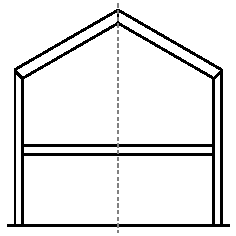
\includegraphics[height=4cm]{mirror_symmetry.pdf}
%	\caption{Simetría bilateral.}
%	\end{subfigure}
%    \begin{subfigure}[b]{0.49\textwidth}
%    \centering
%	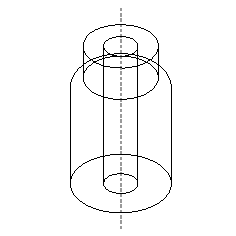
\includegraphics[height=4cm]{axial_symmetry.pdf}
%	\caption{Simetría rotacional.}
%	\end{subfigure}\\	
%	\begin{subfigure}[b]{0.49\textwidth}
%	\centering
%	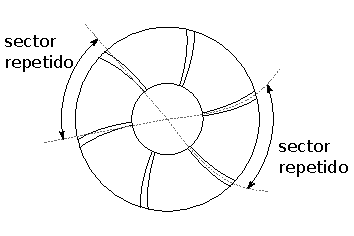
\includegraphics[height=4cm]{cyclic_symmetry.pdf}
%	\caption{Simetría cíclica.}
%	\end{subfigure}
%    \begin{subfigure}[b]{0.49\textwidth}
%    \centering
%	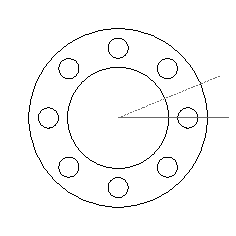
\includegraphics[height=4cm]{cyclic-mirror_symmetry.pdf}
%	\caption{Simetría cíclica/bilateral.}
%	\end{subfigure}\\
%    \begin{subfigure}[b]{\textwidth}
%    \centering
%	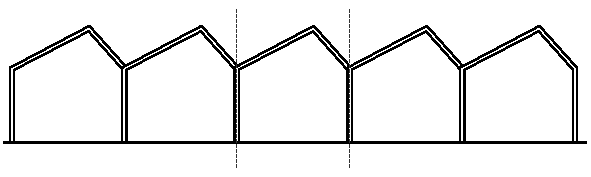
\includegraphics[height=3cm]{repetitive_symmetry.pdf}
%	\caption{Simetría repetitiva.}
%	\end{subfigure}\\
%    \begin{subfigure}[b]{\textwidth}
%    \centering
%	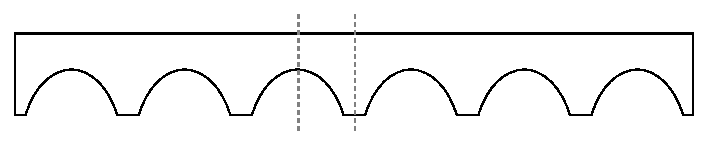
\includegraphics[height=2.5cm]{repetitive-mirror_symmetry.pdf}
%	\caption{Simetría repetitiva/bilateral.}
%	\end{subfigure}
%    \caption{Tipos de simetrías en diferentes geometrías \cite{how_to_FEM}.}
%    \label{fig:simetrias}
%\end{figure}

%%% Ejemplo con SolidsPy

%\section{Creación y solución de un modelo de elementos finitos paso a paso}
%Esta sección incluye un tutorial sobre cómo generar una geometría (específica) 
%usando Gmsh y su posterior procesamiento para la generación de archivos de 
%entrada para un programa de Elementos Finitos en Python\footnote{El programa 
%de 
%elementos finitos trabajado en clase escrito en Python que puede descargarse 
%del sitio \url{https://github.com/AppliedMechanics-EAFIT/SolidsPy}.}.
%
%\subsection{Modelo a resolver}
%El ejemplo que se piensa resolver corresponde con la determinación de 
%esfuerzos en un cilindro en la \emph{Prueba Brasilera}. La Prueba Brasilera  
%es 
%una técnica que se usa para la medida indirecta de la resistencia de rocas. Es 
%una técnica simple y efectiva, y por ello es comúnmente usada para medidas de 
%rocas. En algunas ocasiones esta prueba se usa también para concreto 
%\cite{brazilian_test}.
%
%La siguiente figura presenta un esquema del modelo a resolver. Ya que el 
%modelo original puede presentar desplazamientos de cuerpo rígido, se decide 
%utilizar la simetría del problema. Entonces, el problema a resolver es un 
%cuarto del problema original y las superficies inferior e izquierda presentan 
%restricciones de \emph{rodillo}.
%\begin{figure}[H]
%    \centering
%    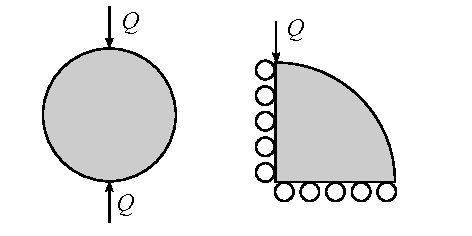
\includegraphics[height=6cm]{Prueba_brasilera.pdf}
%    \caption{Esquema del modelo a resolver. A la derecha se presenta una 
%versión de la geometría simplificada, debido a las simetrías del problema.}
%\end{figure}
%
%\subsection{Generación de la geometría y malla en Gmsh}
%Como primer paso, se sugiere crear un nuevo archivo en Gmsh, como se muestra 
%en la siguiente figura.
%\begin{figure}[H]
%    \centering
%    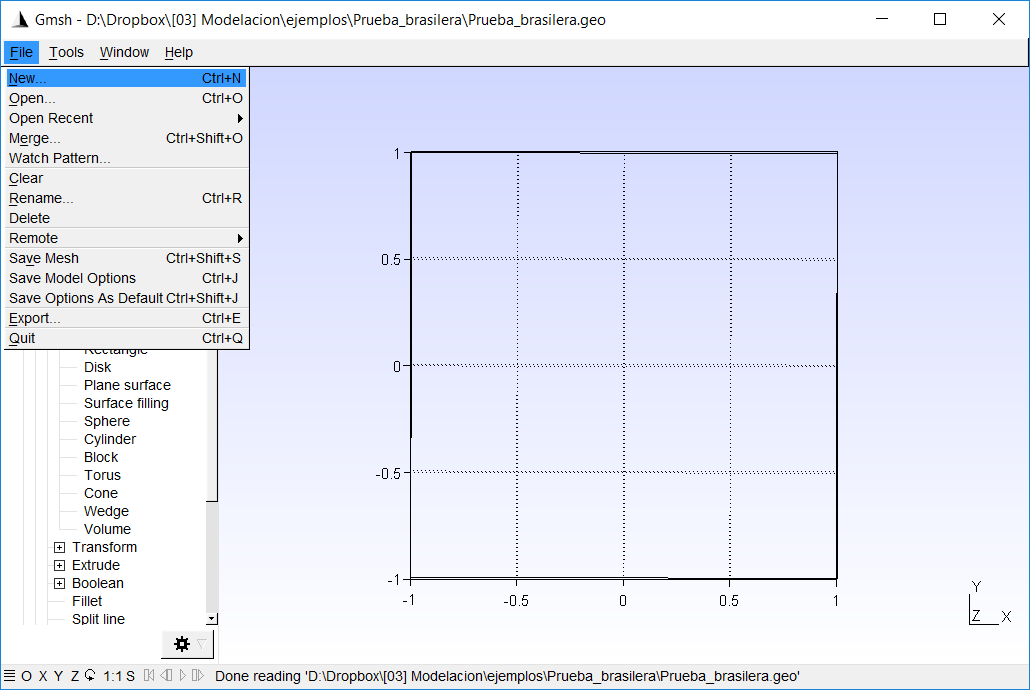
\includegraphics[height=8cm]{Nuevo_archivo.png}
%    \caption{Creación de nuevo archivo en Gmsh.}
%\end{figure}
%
%Al crear un nuevo documento es posible\footnote{Si la versión es 3.0 o mayor, 
%esta ventana emergente aparecerá} que Gmsh pregunte sobre cuál motor 
%geométrico 
%usar. No nos detendremos en cuáles son las diferencias y usaremos 
%\texttt{built-in}.
%\begin{figure}[H]
%    \centering
%    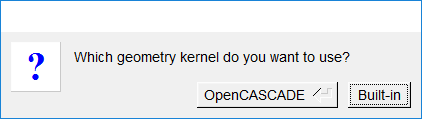
\includegraphics[height=2cm]{Motor_geometrico.png}
%    \caption{Ventana emergente preguntando por el motor geométrico.}
%\end{figure}
%
%Para crear un modelo, inicialmente creamos los puntos. Para ello, vamos a la 
%opción: \texttt{Geometry > Elementary Entities > Add > Point}, como se muestra 
%en la siguiente figura. Luego, se añaden las coordenadas de los puntos en la 
%ventana emergente y ``Add''. Para finalizar podemos cerrar la ventana 
%emergente 
%y presionar \texttt{e}.
%\begin{figure}[H]
%    \centering
%    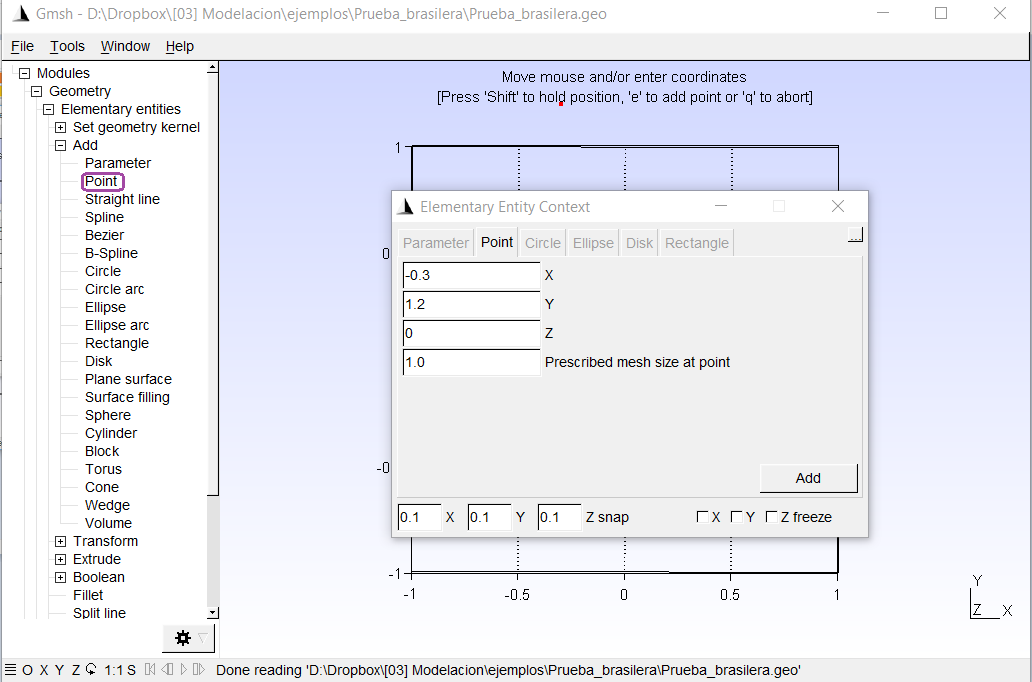
\includegraphics[height=8cm]{Agregar_puntos.png}
%    \caption{Agregar puntos al modelo.}
%\end{figure}
%
%Posteriormente creamos líneas. Para ello, vamos a la opción: \texttt{Geometry 
%> Elementary Entities > Add > Straight line}, como se muestra en la siguiente 
%figura, y seleccionamos los puntos iniciales y finales para cada línea. Al 
%finalizar, podemos presionar \texttt{e}.
%\begin{figure}[H]
%    \centering
%    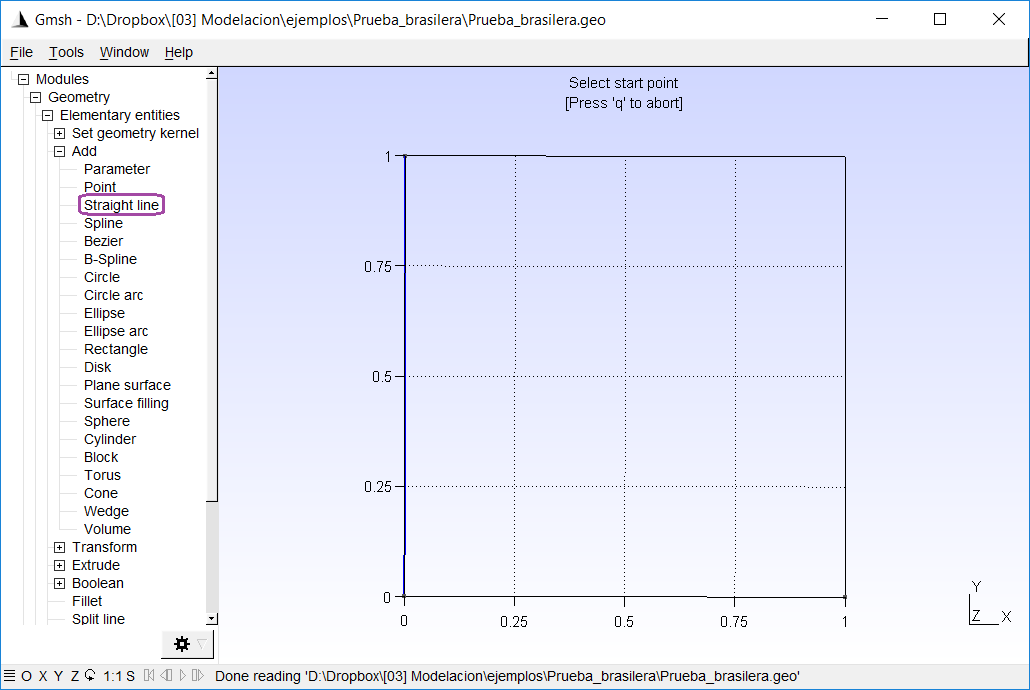
\includegraphics[height=8cm]{Agregar_lineas.png}
%    \caption{Agregar líneas rectas al modelo.}
%\end{figure}
%
%También creamos los arcos de circunferencia. Para ello, vamos a la opción: 
%\texttt{Geometry > Elementary Entities > Add > Circle Arc}, como se muestra en 
%la siguiente figura, y seleccionamos los puntos iniciales, centrales y finales 
%para cada arco (en ese orden). Al finalizar, podemos presionar \texttt{e}.
%\begin{figure}[H]
%    \centering
%    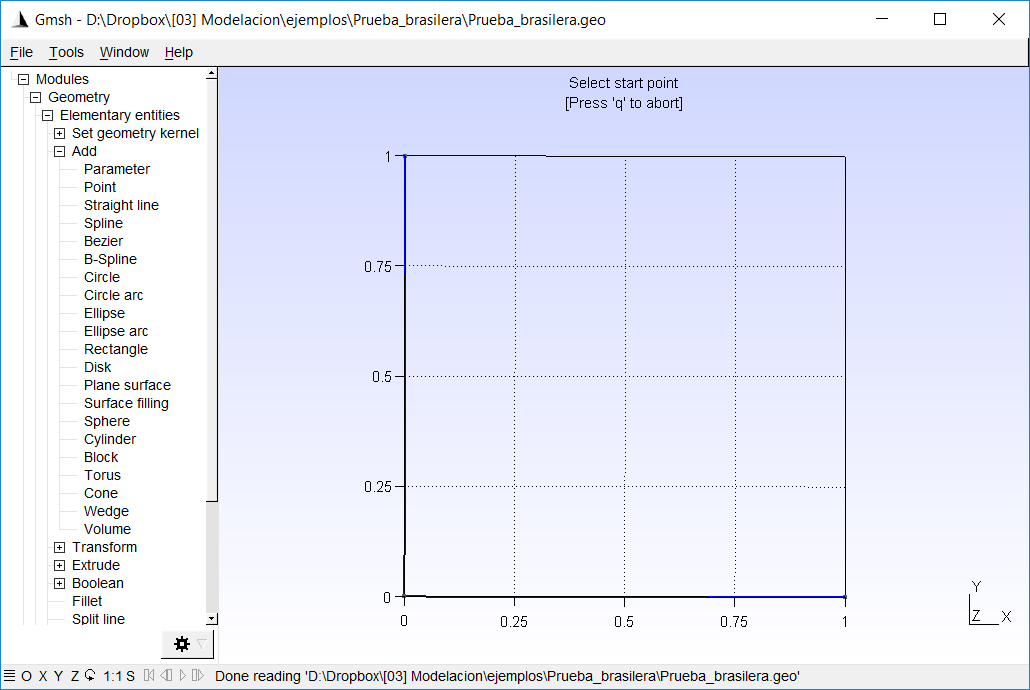
\includegraphics[height=8cm]{Agregar_arcos.png}
%    \caption{Agregar arcos al modelo.}
%\end{figure}
%
%Como ya tenemos un contorno cerrado, podemos definir una superficie. Para 
%ello, vamos a la opción: \texttt{Geometry > Elementary Entities > Add > Plane 
%Surface}, como se muestra en la siguiente figura, y seleccionamos los 
%contornos 
%en orden. Al finalizar, podemos presionar \texttt{e}.
%\begin{figure}[H]
%    \centering
%    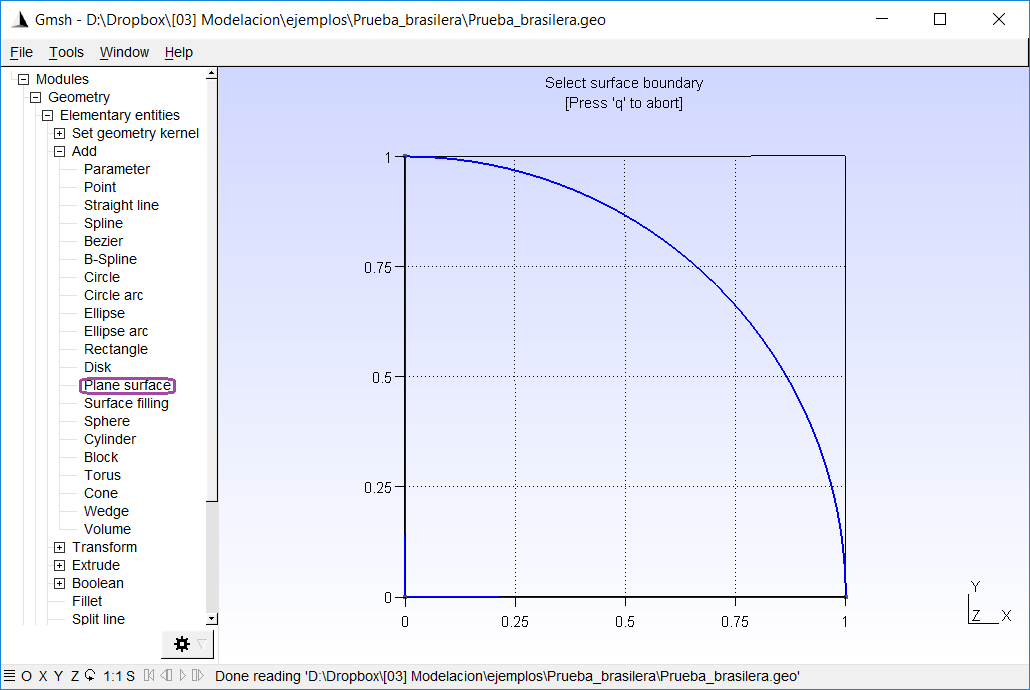
\includegraphics[height=8cm]{Agregar_superficie.png}
%    \caption{Agregar superficies al modelo.}
%\end{figure}
%
%Ahora, necesitamos definir \emph{grupos físicos}. Los grupos físicos permiten 
%asociar nombres a diferentes partes del modelo como líneas y superficies. Esto 
%nos permitirá definir la región en la que resolveremos el modelo (y 
%asociaremos 
%un material), las regiones que tienen desplazamientos restringidos 
%(condiciones 
%de frontera) y las regiones sobre las que aplicaremos la carga. En nuestro 
%caso 
%tendremos 4 grupos físicos:
%\begin{itemize}
%    \item Región del modelo, en donde definiremos un material;
%    \item Borde inferior, en donde restringiremos el desplazamiento en $y$;
%    \item Borde izquierdo, en donde restringiremos el desplazamiento en $x$; y
%    \item Punto superior, en donde aplicaremos la carga puntual.
%\end{itemize}
%
%Para definir los grupos físicos vamos a  \texttt{Geometry > Physical groups > 
%Add > Plane Surface}, como muestra la siguiente figura. En este caso, podemos 
%dejar el campo de \texttt{Name} vacío y permitir que Gmsh nombre los grupos 
%por 
%nosotros, los cuales serán números que luego podemos consultar en el archivo 
%de 
%texto.
%\begin{figure}[H]
%    \centering
%    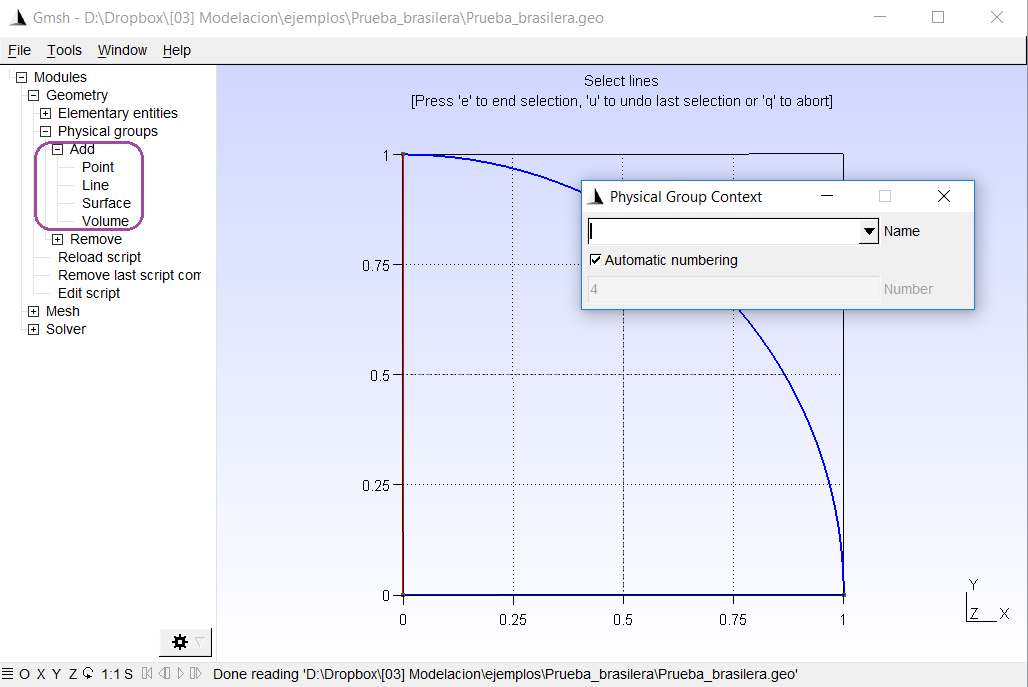
\includegraphics[height=8cm]{Agregar_linea_fisica.png}
%    \caption{Agregar grupos físicos al modelo.}
%\end{figure}
%
%Luego de editar ligeramente, el archivo de texto (.geo) este luce de la 
%siguiente manera. Agregamos un parámetro \texttt{L}, que podremos variar a 
%nuestro antojo para cambiar el tamaño de los elementos al crear la malla.
%\begin{listing}[H]
%    \inputminted[mathescape,
%    linenos,
%    numbersep=5pt,
%    gobble=0,
%    frame=lines,
%    framesep=2mm]{c}{src/tutorial/Prueba_brasilera.geo}
%    \caption{Archivo \texttt{.geo} para el modelo descrito.}
%    \label{lst:geo}
%\end{listing}
%
%Ahora, procedemos a crear la malla. Para ello,  vamos a \texttt{Mesh > 2D}.  
%Como vemos en la figura a continuación.
%\begin{figure}[H]
%    \centering
%    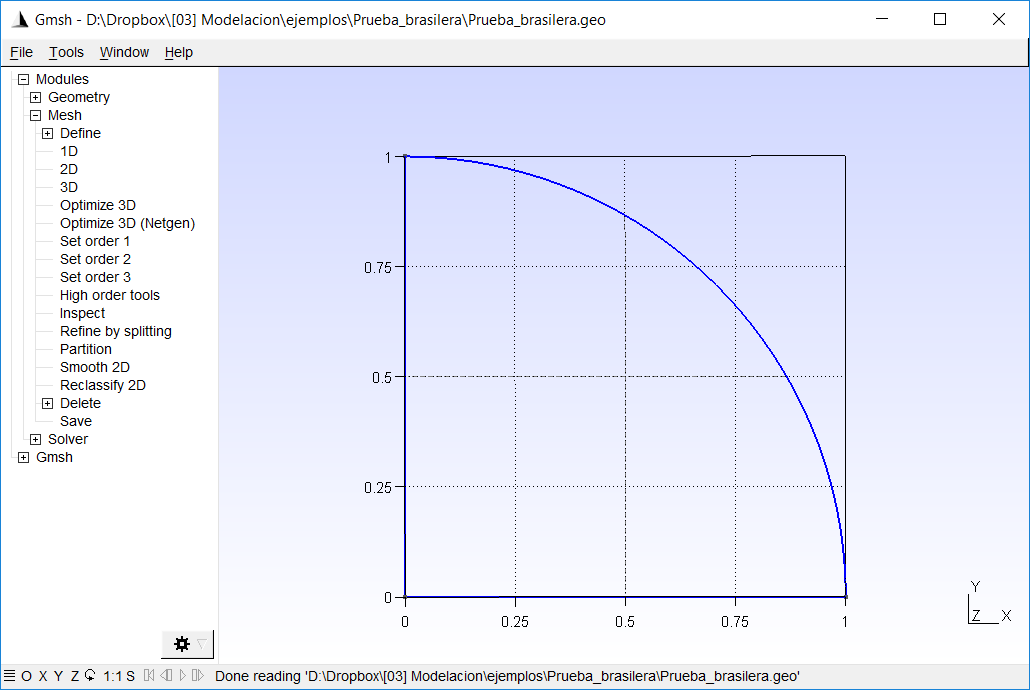
\includegraphics[height=8cm]{Mallar_2D.png}
%    \caption{Crear la malla del modelo.}
%\end{figure}
%
%Adicionalmente, podemos cambiar la configuración para que muestre en colores, 
%los elementos de la malla. Para ello, vamos a \texttt{Tools > Options > Mesh} 
%y 
%marcamos el cuadro que indica \texttt{Surface faces}.
%\begin{figure}[H]
%    \centering
%    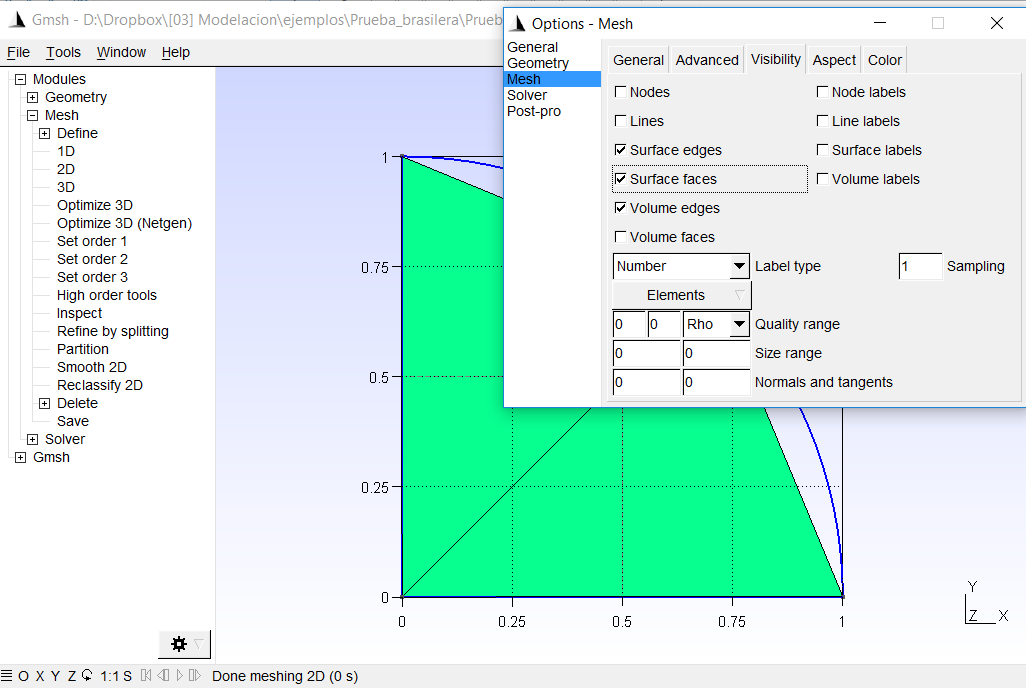
\includegraphics[height=8cm]{Ver_superficie_malla.png}
%    \caption{Crear la malla del modelo.}
%\end{figure}
%
%Podemos entonces refinar la malla yendo a \texttt{Mesh > Refine by Splitting}, 
%o midificando el parámetro \texttt{L} en el archivo de entrada (.geo). Como 
%último paso, queremos salvar la malla. Para ello, vamos a \texttt{Mesh > 
%Save}, 
%o \texttt{File > Save Mesh}, como se muestra a continuación.
%\begin{figure}[H]
%    \centering
%    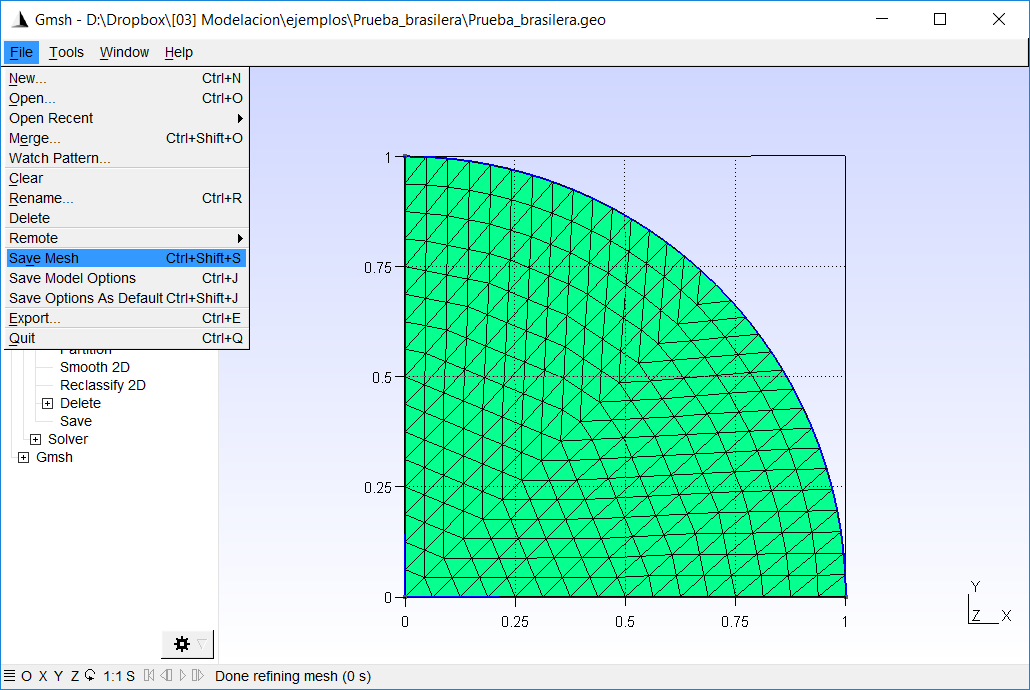
\includegraphics[height=8cm]{Grabar_malla.png}
%    \caption{Guardar la malla a un archivo \texttt{.msh}.}
%\end{figure}
%
%
%
%\section{Conversión a archivos de texto}
%Debemos crear archivos con la información de los nodos (\texttt{nodes.txt}), 
%elementos (\texttt{eles.txt}), cargas (\texttt{loads.txt}) y materiales 
%(\texttt{mater.txt}).
%
%El siguiente código genera los archivos de entrada necesarios para correr el 
%programa de elementos finitos en Python.
%\inputminted[mathescape,
%linenos,
%numbersep=5pt,
%gobble=0,
%frame=lines,
%framesep=2mm]{python}{src/tutorial/Prueba_brasilera_input.py}
%
%
%Ahora, comentemos las diferentes partes del código para ver qué hace cada una.
%
%\subsection{Encabezado y lectura de archivo \texttt{.msh}}
%La primera parte carga los módulos de Python necesarios y lee el archivo de 
%malla que en este caso se llama \texttt{Prueba\_brasilera.msh} (línea 6 y 7). 
%Para que Python sea capaz de leer el archivo, este debe estar en el mismo 
%directorio que el archivo de Python que lo procesará.
%\begin{minted}[mathescape,
%linenos,
%numbersep=5pt,
%gobble=0,
%frame=lines,
%framesep=2mm]{python}
%from __future__ import division, print_function
%import meshio
%import numpy as np
%
%
%points, cells, point_data, cell_data, field_data = \
%meshio.read("Prueba_brasilera.msh")
%\end{minted}
%
%\subsection{Datos de elementos}
%La siguiente sección del código crea los datos para elementos. La línea 18 
%crea una variable \texttt{eles} con la información de los nodos que conforman 
%cada triángulo. La línea 19 crea un arreglo (lleno de ceros) con la cantidad 
%de 
%filas igual al número de elementos (\mintpy{eles.shape[0]}) y 6 
%columnas\footnote{Para elementos cuadriláteros se utilizarían 7 columnas, pues 
%cada elemento está definido por 4 nodos.}. Luego asignamos un número a cada 
%elemento, esto lo hacemos en la línea 20 con \mintpy{range(eles.shape[0])} y 
%esto lo asignamos a la columna 0. Todos los materiales son triángulos, por eso 
%debemos poner 3 en la columna 1. Por último, en esta sección, asignamos los 
%nodos de cada elemento al arreglo con \mintpy{els_array} (línea 22), y esta 
%asignación la hacemos desde la columna 3 hasta el final con 
%\mintpy{els_array[:, 3::]}.
%\begin{minted}[mathescape,
%linenos,
%numbersep=5pt,
%gobble=0,
%frame=lines,
%framesep=2mm,
%firstnumber=17]{python}
%# Datos elementales
%eles = cells["triangle"]
%els_array = np.zeros([eles.shape[0], 6], dtype=int)
%els_array[:, 0] = range(eles.shape[0])
%els_array[:, 1] = 3
%els_array[:, 3::] = eles
%\end{minted}
%
%\subsection{Datos de nodos}
%En la siguiente sección creamos la información relacionada con los nodos. Para 
%ello, en la línea 25 creamos un arreglo \mintpy{nodes_array} con 5 columnas y 
%tantas filas como puntos tenemos en el modelo (\mintpy{point.shape[0]}). 
%Luego, 
%asignamos el número de elemento en la línea 26. Y, por último, asignamos la 
%información de las coordenadas de los nodos en la línea 27 con 
%\mintpy{nodes_array[:, 1:3] = points[:, :2]}, en donde estamos poniendo la 
%información en las columnas 1 y 2.
%\begin{minted}[mathescape,
%linenos,
%numbersep=5pt,
%gobble=0,
%frame=lines,
%framesep=2mm,
%firstnumber=24]{python}
%# Nodos
%nodes_array = np.zeros([points.shape[0], 5])
%nodes_array[:, 0] = range(points.shape[0])
%nodes_array[:, 1:3] = points[:, :2]
%\end{minted}
%
%\subsection{Datos de Fronteras}
%En la siguiente sección encontramos la información de líneas. Para esto, 
%leemos la información de \mintpy{cells} en la posición 
%\mintpy{"line"}\footnote{\mintpy{cells} es un diccionario y permite almacenar 
%información asociada a unas palabras clave, en este caso es \mintpy{"lines"}.} 
%(línea 30). El arreglo resultante \mintpy{lines} tendrá, entonces, la 
%información de los nodos que forman cada línea que está en la frontera del 
%modelo. Luego, leemos la información de las líneas físicas (línea 31), y 
%calculamos cuántas líneas pertenecen a las líneas físicas (línea 32).
%\begin{minted}[mathescape,
%linenos,
%numbersep=5pt,
%gobble=0,
%frame=lines,
%framesep=2mm,
%firstnumber=30]{python}
%# Fronteras
%lines = cells["line"]
%bounds = cell_data["line"]["physical"]
%nbounds = len(bounds)
%\end{minted}
%
%\subsection{Datos de carga}
%En la siguiente sección debemos definir la información de cargas, en este 
%caso, las cargas las asignamos en un único punto que definimos como grupo 
%físico. En la línea 31 leemos los nodos (en este caso, uno). Luego, creamos un 
%arreglo que tiene tantas filas como cargas (\mintpy{nloads}) y 3 columnas. 
%Asignamos el número del nodo al que pertenece cada carga (línea 35, las cargas 
%en $x$ (línea 36) y las cargas en $y$ (línea 37).
%\begin{minted}[mathescape,
%linenos,
%numbersep=5pt,
%gobble=0,
%frame=lines,
%framesep=2mm,
%firstnumber=30]{python}
%# Cargas
%id_cargas = cells["vertex"]
%nloads = len(id_cargas)
%load = -10e8 # N/m
%loads_array = np.zeros((nloads, 3))
%loads_array[:, 0] = id_cargas
%loads_array[:, 1] = 0
%loads_array[:, 2] = load
%\end{minted}
%
%\subsection{Condiciones de frontera}
%Ahora, procederemos a aplicar las condiciones de frontera, es decir, las 
%regiones del modelo que tienen restricciones en el desplazamiento. 
%Inicialmente, identificamos cuáles líneas tienen como identificador 1 (que 
%serían las del lado izquierdo) con
%
%\mint{python}{id_izq = [cont for cont in range(nbounds) if bounds[cont] == 1]}
%
%Esto crea una lista con los números (\mintpy{cont}) para los cuales se cumple 
%la condición (\mintpy{bounds[cont] == 1}). Ahora, en la línea 46 obtenemos los 
%nodos que pertenecen a estas líneas, sin embargo, este arreglo tiene tantas 
%filas como líneas en el lado izquierdo y dos columnas. Primero volvemos este 
%arreglo como un arreglo unidimensional con \mintpy{nodes_izq.flatten()}. 
%Posteriormente, en la línea 50, asignamos el valor de -1 en la tercera columna 
%del arreglo \mintpy{nodes_array} para los nodos que pertenezcan al lado 
%izquierdo. De igual forma, se repite este proceso para los nodos en la 
%frontera 
%inferior.
%\begin{minted}[mathescape,
%linenos,
%numbersep=5pt,
%gobble=0,
%frame=lines,
%framesep=2mm,
%firstnumber=30]{python}
%# Condiciones de frontera
%id_izq = [cont for cont in range(nbounds) if bounds[cont] == 1]
%id_inf = [cont for cont in range(nbounds) if bounds[cont] == 2]
%nodes_izq = lines[id_izq]
%nodes_izq = nodes_izq.flatten()
%nodes_inf = lines[id_inf]
%nodes_inf = nodes_inf.flatten()
%nodes_array[nodes_izq, 3] = -1
%nodes_array[nodes_inf, 4] = -1
%\end{minted}
%
%\subsection{Materiales}
%En la siguiente sección asignamos los materiales correspondientes a cada 
%elemento. En este caso, sólo tenemos un material. Sin embargo, se presenta el 
%ejemplo como si hubieran dos diferentes.  Primero, creamos un arreglo con la 
%información de materiales en donde la primera columna representa el módulo de 
%Young y la segunda la relación de Poisson (línea 54). Luego, leemos la 
%información de los grupos físicos de superficies en la línea 56. Finalmente, 
%asignamos el valor de 0 a los materiales que tengan como grupo físico 4 (ver 
%archivo \texttt{.geo} arriba) y 1 a los otros, que en este caso serán cero 
%(línea 57). Esta información va en la columna 2 del arreglo \mintpy{els_array}.
%\begin{minted}[mathescape,
%linenos,
%numbersep=5pt,
%gobble=0,
%frame=lines,
%framesep=2mm,
%firstnumber=30]{python}
%#  Materiales
%mater_array = np.array([[186e9, 0.29],
%[70e9, 0.35]])
%maters = cell_data["triangle"]["physical"]
%els_array[:, 2]  = [0 if mater == 4 else 1 for mater in maters]
%\end{minted}
%
%\subsection{Escritura de archivos}
%La última sección usa la función \mintpy{savetxt} de \texttt{numpy} para 
%exportar los archivos.
%\begin{minted}[mathescape,
%linenos,
%numbersep=5pt,
%gobble=0,
%frame=lines,
%framesep=2mm,
%firstnumber=30]{python}
%# Generar archivos
%np.savetxt("eles.txt", els_array, fmt="%d")
%np.savetxt("nodes.txt", nodes_array,
%fmt=("%d", "%.4f", "%.4f", "%d", "%d"))
%np.savetxt("loads.txt", loads_array, fmt=("%d", "%.6f", "%.6f"))
%np.savetxt("mater.txt", mater_array, fmt="%.6f")
%\end{minted}
%
%
%\subsection{Solución del modelo por Elementos Finitos}
%Para resolver el modelo se debe ejecutar el programa 
%\texttt{solids\_GUI.py}\footnote{Para hacer uso de la interfaz gráfica debe 
%estar instalado \texttt{eaygui}.}. Luego de correr este programa aparecerá una 
%ventana emergente como se muestra a continuación. En esta ventana emergente se 
%debe ubicar el directorio en donde están los archivos de entrada generados 
%anteriormente. Tenga en cuenta que la apariencia de esta ventana puede variar 
%entre sistemas operativos. También tenga en cuenta que en algunas ocasiones la 
%ventana emergente puede quedar oculta por otras ventanas en su escritorio.
%\begin{figure}[H]
%    \centering
%    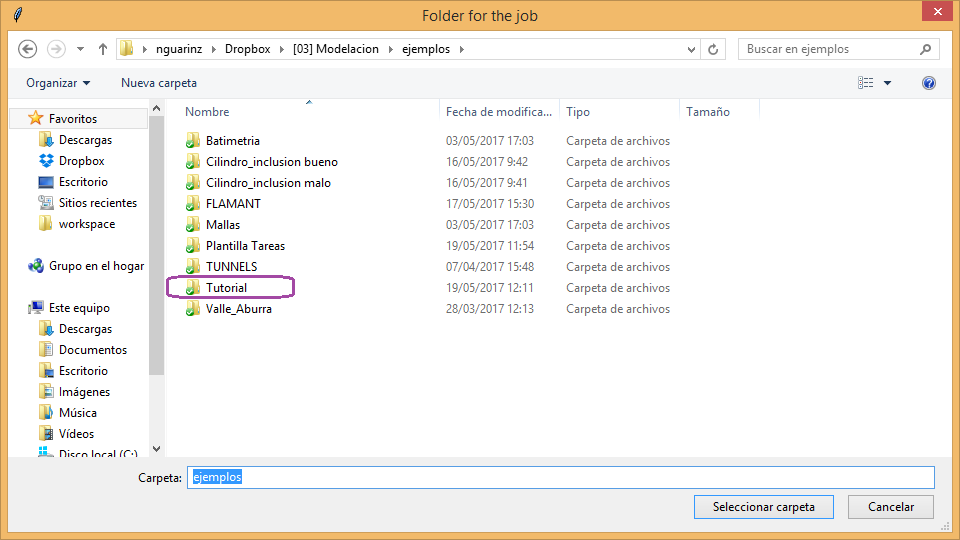
\includegraphics[height=5cm]{solids_ISO-ventana.png} 
%    \caption{Ventana emergente para ubicar el directorio con los archivos de 
%entrada.}
%\end{figure}
%
%En este punto, el programa debe resolver su modelo. Si se usan los archivos de 
%entrada sin modificaciones el programa debe imprimir lo siguiente en la 
%consola 
%de Python
%\begin{verbatim}
%Number of nodes: 123
%Number of elements: 208
%Number of equations: 224
%Duration for system solution: 0:00:00.086983
%Duration for post processing: 0:00:00
%Analysis terminated successfully!
%\end{verbatim}
%los tiempos que se toma en solucionar el sistema pueden cambiar un poco de un 
%computador a otro.
%
%Como último paso, el programa genera unos gráficos con los campos de 
%desplazamientos, deformaciones y esfuerzos, como se muestra en la siguiente 
%figura.
%\begin{figure}[H]
%    \centering
%    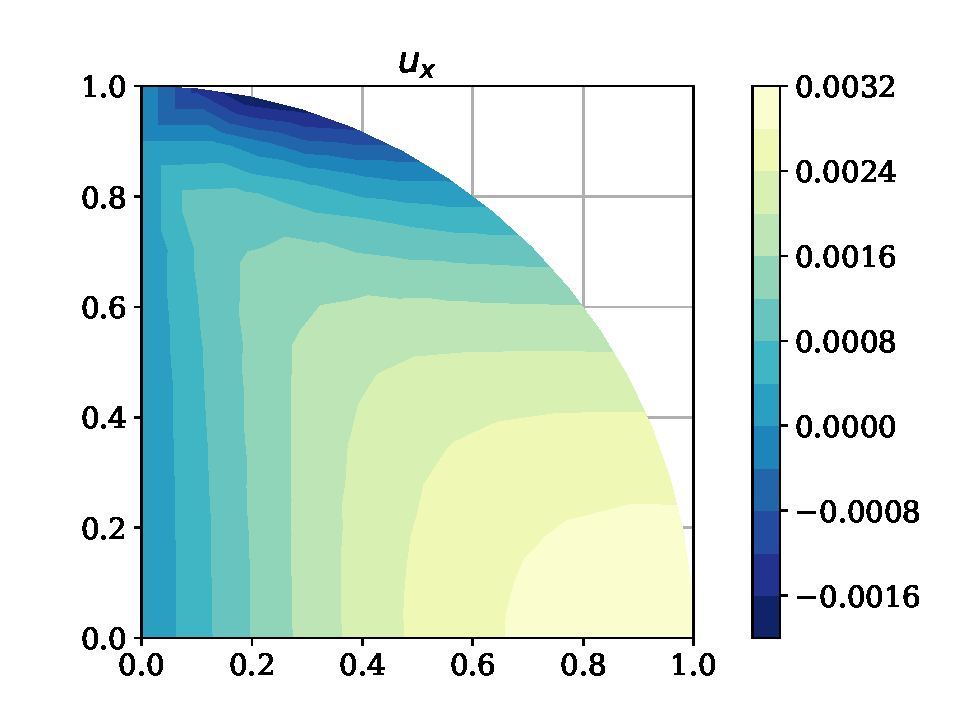
\includegraphics[height=5cm]{Prueba_brasilera_ux.pdf} 
%    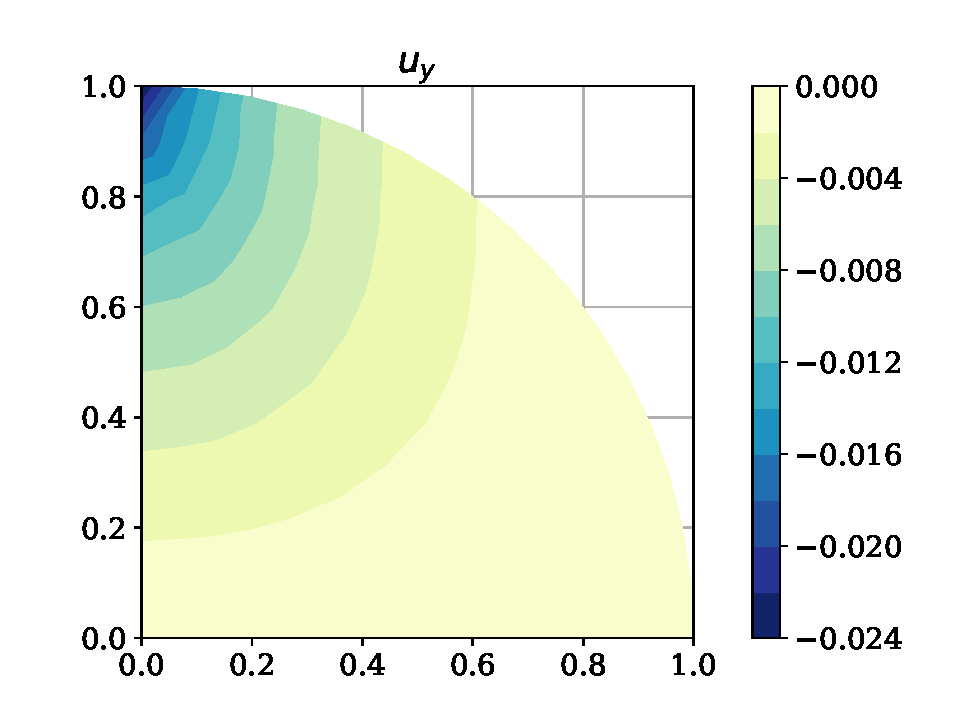
\includegraphics[height=5cm]{Prueba_brasilera_uy.pdf}
%    \caption{Solución de desplazamientos para el modelo. \textbf{(Izquierda)} 
%Desplazamientos horizontales.
%    \textbf{(Derecha)} Desplazamientos verticales.}
%\end{figure}
%
%
%\section{Ejemplo de archivos de entrada para una malla sencilla}
%Supongamos que tenemos un cuadrado de lado 1, con dos cargas en los nodos 
%superiores y los nodos inferiores empotrados, y que está hecho de acero 1020, 
%el cual tiene un módulo de Young $E = 186$ GPa y una relación de Poisson de 
%$\nu = 0.29$.
%
%Si subdividimos el cuadrado en dos triángulos, tendríamos como archivos de 
%entrada
%\begin{listing}[H]
%    \begin{minted}[mathescape,
%               linenos,
%               numbersep=5pt,
%               gobble=4,
%               frame=lines,
%               framesep=2mm]{python}
%    0  0.0  0.0 -1 -1
%    1  1.0  0.0 -1 -1
%    2  1.0  1.0  0  0
%    3  1.0  0.0  0  0
%    \end{minted}
%    \caption{Archivo \texttt{nodes.txt}.}
%    \label{lst:nodes}
%\end{listing}
%
%
%\begin{listing}[H]
%    \begin{minted}[mathescape,
%               linenos,
%               numbersep=5pt,
%               gobble=4,
%               frame=lines,
%               framesep=2mm]{python}
%    0  3  0  0  1  3 
%    1  3  0  1  2  3
%    \end{minted}
%    \caption{Archivo \texttt{eles.txt}.}
%    \label{lst:elements}
%\end{listing}
%
%\begin{listing}[H]
%    \begin{minted}[mathescape,
%               linenos,
%               numbersep=5pt,
%               gobble=4,
%               frame=lines,
%               framesep=2mm]{python}
%    2  1  1
%    3  1  1
%    \end{minted}
%    \caption{Archivo \texttt{loads.txt}.}
%    \label{lst:loads}
%\end{listing}
%
%\begin{listing}[H]
%    \begin{minted}[mathescape,
%               linenos,
%               numbersep=5pt,
%               gobble=4,
%               frame=lines,
%               framesep=2mm]{python}
%    185e9  0.29
%    \end{minted}
%    \caption{Archivo \texttt{mater.txt}.}
%    \label{lst:mater}
%\end{listing}
%
%Si quisiéramos generar esta malla a partir de Gmsh, tendríamos como archivo 
%\texttt{.geo}:
%\begin{listing}[H]
%	\inputminted[mathescape,
%               linenos,
%               numbersep=5pt,
%               gobble=0,
%               frame=lines,
%               framesep=2mm]{c}{src/tutorial/Cuadrado.geo}
%    \caption{Archivo \texttt{Cuadrado.geo}.}
%    \label{lst:mater}
%\end{listing}
